% THIS IS AN EXAMPLE DOCUMENT FOR VLDB 2012
% based on ACM SIGPROC-SP.TEX VERSION 2.7
% Modified by  Gerald Weber <gerald@cs.auckland.ac.nz>
% Removed the requirement to include *bbl file in here. (AhmetSacan, Sep2012)
% Fixed the equation on page 3 to prevent line overflow. (AhmetSacan, Sep2012)
%Ideas for the future: separate computing time for counts from ct-table.
%Reorganize so we don't use the term "nodes" and introduce Bayes nets later.

\documentclass{vldb}
\usepackage{array}
\newcolumntype{R}[1]{>{\raggedleft\let\newline\\\arraybackslash\hspace{0pt}}m{#1}}

\usepackage{graphicx}

%Preamble File for Random Regression Paper

%\usepackage{times}

%Theorems and such

%\usepackage{amsthm}

%\newtheorem{theorem}{Theorem}
%\newtheorem{observation}{Observation}
%\newtheorem{proposition}{Proposition}
%\newtheorem{definition}{Definition}

%\newtheorem{theorem}{Theorem}[section]
%\newtheorem{observation}{Observation}[section]
%\newtheorem{proposition}{Proposition}[section]
%\newtheorem{definition}{Definition}[section]

\usepackage[ruled,vlined]{algorithm2e}
\usepackage{algorithmic}
%\usepackage{amsthm}
\usepackage{amsmath}
\usepackage{amsfonts}
\usepackage{amssymb}
\usepackage{graphicx}
\usepackage{url}
\usepackage{subfigure}
\usepackage{epstopdf}
%\setcounter{MaxMatrixCols}{30}
%\usepackage[ruled,vlined]{algorithm2e}
%\usepackage{algorithmic}
\usepackage{multirow}
\usepackage{subfigure}
\usepackage{ifthen}
\DeclareMathOperator*{\argmax}{argmax}
\DeclareMathOperator*{\argmin}{argmin}
%\DeclareMathOperator{\pattern}{\pi}
\DeclareMathOperator{\Poly}{\mathbf{\mathrm{P}}}
\DeclareMathOperator{\RP}{\mathbf{\mathrm{RP}}}
%\DeclareMathOperator{\FP}{\mathbf{\mathrm{FP}}}
\DeclareMathOperator{\NP}{\mathbf{\mathrm{NP}}}
%\DeclareMathOperator{\E}{\mathbb{E}}

\newcommand{\defterm}{\textbf}

\renewcommand{\d}{\mathbf{d}}

\newcommand{\ZZ}{\mathbf{Z}}

\newcommand{\indep}{\ensuremath{\perp{}\!\!\!\!\!\!\!\perp{}}}
\newcommand{\dep}{\ensuremath{{\perp{}\!\!\!\!\!\!\!\not  \perp{}}}}
%\renewcommand{\L}{\mathcal{L}}

% variables denoting sets of nodes
\newcommand{\BN}{B} % Bayes net
\newcommand{\V}{V} 
\newcommand{\partC}{\mathcal{C}}
\newcommand{\pattern}{\pi}
% for population variables
\newcommand{\A}{\mathbb{A}}
\newcommand{\B}{\mathbb{B}}
\newcommand{\C}{\mathbb{C}}
\newcommand{\U}{\mathbb{U}}
%maybe use P, R as well??
\renewcommand{\P}{P}
\newcommand{\R}{R}
% values of Pop variables = constants
\renewcommand{\a}{a}
\renewcommand{\b}{b}
\renewcommand{\c}{c}

%%%
% for terms = nodes in Functor Bayes Net.
\newcommand{\X}{X}
\newcommand{\Y}{Y}
\newcommand{\Z}{Z}
% Next three are currently only ones eligible for \Mrange and \Prange
\newcommand{\TT}{T}
\newcommand{\TI}{\mathsf{T}}
\newcommand{\UT}{U}
\newcommand{\UI}{\mathsf{U}}
\newcommand{\VT}{V}
\newcommand{\VI}{\mathsf{V}}
\newcommand{\W}{W}
%syntax for values
\newcommand{\z}{z}
\renewcommand{\v}{v}
\newcommand{\x}{x}
\newcommand{\y}{y}
\newcommand{\p}{p}
\newcommand{\s}{s}
% Values tied to terms
\newcommand{\TV}{t}
\newcommand{\TTuple}[1][0.0ex]{\vec{t}\hspace{#1}}
\newcommand{\UV}{u}
\newcommand{\UTuple}[1][0.0ex]{\vec{u}\hspace{#1}}
\newcommand{\VV}{v}
\newcommand{\VTuple}{\vec{v}}
%%%
\newcommand{\weight}{w} % weights
% Formulas
\newcommand{\TF}{\vec{T}}
\newcommand{\UF}{\vec{U}}
\newcommand{\VF}{\vec{V}}
%\newcommand{\TF}{\phi}
%\newcommand{\UF}{\psi}
%\newcommand{\VF}{\omega}
% Database (which is always fully-grounded)
\newcommand{\DB}{\FG{\Delta}}
\newcommand{\QC}{\FG{\Lambda}}
\newcommand{\QCtarget}{\FG{\Lambda_{-\TI}}}
% to define a query conjunction of literals
\newcommand{\Qconj}{\Appendterm{\FG{\TT_{\grounding}} = \TV} {\QC}}

% Annotations marking degree of grounding
\newcommand{\UG}[2][0.0ex]{#2^{-}\hspace{#1}}
\newcommand{\PG}[2][0.0ex]{#2^{\prime}\hspace{#1}}
\newcommand{\FG}[2][0.0ex]{#2^{*}\hspace{#1}}

% Functions returning related terms
\newcommand{\MB}[1]{\mathrm{MB}(#1)}
\newcommand{\Pa}[1]{\mathrm{Pa}(#1)}
\newcommand{\Ch}[1]{\mathrm{Ch}(#1)}

% Grounding
\newcommand{\Ground}[1]{#1_\gamma}
\newcommand{\gndlink}{\backslash}

% Values in ranges of example functors
\newcommand{\Man}{\mathrm{M}}
\newcommand{\Woman}{\mathrm{W}}

% Adding a term to a formula
\newcommand{\sepcup}[1][0.5ex]{\hspace{#1}\cup\hspace{#1}}
\newcommand{\Setaddterm}[2]{#1 \sepcup #2}
\newcommand{\Appendterm}[2]{#1, #2}

% Values in the range of related terms
\newcommand{\Mrange}[1]{\ifthenelse{\equal{#1}{T}}{\TTuple_m}{\ifthenelse{\equal{#1}{U}}{\UTuple_m}{\ifthenelse{\equal{#1}{V}}{\VTuple_m}{\mbox{UNKNOWN
TERM ID}}}}}
\newcommand{\Prange}[1]{\ifthenelse{\equal{#1}{T}}{\vec{t}_{pa}}{\ifthenelse{\equal{#1}{U}}{\vec{u}_{pa}}{\ifthenelse{\equal{#1}{V}}{\vec{v}_{pa}}{\mbox{UNKNOWN
TERM ID}}}}}

\newcommand{\GroundPrange}[1]{\ifthenelse{\equal{#1}{T}}{\vec{t}_{pa,\grounding'}}{\ifthenelse{\equal{#1}{U}}{\vec{u}_{pa,\grounding'}}{\ifthenelse{\equal{#1}{V}}{\vec{v}_{pa,\grounding'}}{\mbox{UNKNOWN
TERM ID}}}}}


% Key functions
\newcommand{\joint}{p}
\newcommand{\jprob}[1]{\theta(#1)}
\newcommand{\cprob}[2]{\theta(#1|#2)}
\newcommand{\estcprob}[3]{\widehat{\theta}(#1|#2;#3)}
%\newcommand{\Gpvar}{\tilde{P}}
\newcommand{\Gpvar}{P}
\newcommand{\Gprob}[2]{\Gpvar(#1 | #2)}
\newcommand{\QFC}{QFC} % query family configuration
\newcommand{\Cvar}{\mathrm{n}}
\newcommand{\Fvar}{\mathrm{p}}
\newcommand{\Count}[2]{\Cvar\left[#1;#2\right]}
\newcommand{\CountC}[3]{\Cvar_{#3}\left[#1;#2\right]}
\newcommand{\Freq}[2]{\Fvar\left[#1;#2\right]}
\newcommand{\Relevant}[1]{#1^{\mathrm{r}}}
\newcommand{\Relcount}[2]{\Relevant{\Cvar}\left[#1;#2\right]}
\newcommand{\RelcountC}[3]{\Relevant{\Cvar_{#3}}\left[#1;#2\right]}
\newcommand{\Relfreq}[2]{\Relevant{\Fvar}\left[#1;#2\right]}
\newcommand{\RelfreqC}[3]{\Relevant{\Fvar_{#3}}\left[#1;#2\right]}
\newcommand{\Range}[1]{\mathrm{Ra}(#1)}
\newcommand{\Vars}[1]{\mathrm{Va}(#1)}
% no longer needed
%\newcommand{\Crossprod}[1]{\mathcal{X}}

%variables for sets of values
\newcommand{\setx}{\set{x}}
\newcommand{\sety}{\set{y}}
\newcommand{\setz}{\set{z}}


%statistics
\newcommand{\score}{S}
\newcommand{\parameters}{\mathit{par}}
\newcommand{\bic}{\mathit{BIC}}
%random variables and graphical models
% number of values in the domain of a random variable
% variables for BNs
\newcommand{\domvals}{k}
\newcommand{\nodevalue}{\x}
\newcommand{\parvalue}{\mathbf{\pi}} % a single assignment of values to a set of 
%parents
\newcommand{\parvals}{l} % number of values of parent state.
\renewcommand{\r}{r} % CP-table row
\newcommand{\nbhd}{{\mathsf {nbdh}}}
\newcommand{\child}{\mathit{child}}
\newcommand{\parent}{\mathit{pa}}
\newcommand{\parents}{\mathbf{pa}}
\newcommand{\Parents}{\mathbf{PA}}
\newcommand{\family}{F} % families, family formulas
\newcommand{\Target}{Y_{\target}}
\newcommand{\MBtarget}{\set{X}_{\target}} % Markov blanket of a target node.
\newcommand{\mbtarget}{\set{x}} % values for the markov blanket of a variable, vector-valued
\newcommand{\mbstates}{m} % number of states in Markov blanket
\newcommand{\vpi}{\mathbf{pa}} % for vectors of variable assignments
\renewcommand{\l}{\ell} % class label
\newcommand{\states}{r} % number of states of a variable
\newcommand{\ssize}{N} % number of rows in join table; size of sample
\newcommand{\frequency}{fr}
\newcommand{\pseudo}{\ast}
\newcommand{\counts}{+}
\newcommand{\weighted}{\ast}
\newcommand{\halpern}{H}
\newcommand{\instance}{I}

%logic notation
\newcommand{\functor}{f}
\newcommand{\fvalue}{v}
\newcommand{\variable}{X} % first-order variable
\newcommand{\population}{\mathcal{P}}
\newcommand{\entity}{x}
\newcommand{\formula}{\phi}
\newcommand{\formulas}{\mathcal{\phi}}
\newcommand{\conjunction}{\set{C}} % 
\newcommand{\outdomain}{V}
\newcommand{\literal}{\ell}
%conjunction of literals
\newcommand{\fterm}{\f} % open function term
\newcommand{\fterms}{F} % set of function terms, also nodes in JBN
\newcommand{\term}{\tau}
\newcommand{\terms}{\bs{\tau}}
\newcommand{\constant}{a}
\newcommand{\constants}{\bs{\constant}}
\newcommand{\gterm}{g} % ground term
\newcommand{\gterms}{\bs{\gterm}} %list of ground terms
\newcommand{\vterm}{x} % variable term
\newcommand{\vterms}{\bs{\vterm}} % list of variable terms
\newcommand{\assign}{A} % assignment of values to Bayes net
\newcommand{\grounds}{\#}
\newcommand{\grounding}{\gamma}
\newcommand{\groundall}{\Gamma}
\newcommand{\vars}{\mathit{Var}} % variables in a conjunction
\newcommand{\igraph}{I} % instance-level dependency graph.
\newcommand{\assignment}{\set{a}}
\newcommand{\atom}{\functor}
\newcommand{\gnode}{\alpha}
\newcommand{\gfamily}{\ground{f}}
\newcommand{\numformulas}{m}
% logic programs
\newcommand{\program}{\mathcal{B}}
\newcommand{\clause}{\mathcal{c}}
\newcommand{\head}{\mathit{head}}
\newcommand{\body}{\mathit{body}}
\newcommand{\crule}{\mathit{cr}} % combining rule
\newcommand{\level}{\mathit{level}} % rank of function symbols in LP

%datbase schema
\newcommand{\rcolumns}{R}
\newcommand{\ecolumns}{E}
\newcommand{\dtable}{T} % can't use \table. Generic database table
\newcommand{\datatable}{D} % generic data table, not necessarily part of database.
\newcommand{\jtable}{J} % join table
\newcommand{\Ejoin}{$J^{+}$}
\newcommand{\jtables}{m}
\newcommand{\rtable}{R} % relationship table
\newcommand{\etable}{E} % entity table.
\newcommand{\ttable}{X} % target table
\newcommand{\nextended}{n}
\newcommand{\row}{r}
\newcommand{\rows}{\mathit{rows}}
\newcommand{\col}{j}
\newcommand{\cols}{\mathit{cols}}
\newcommand{\unary}{\f} % to denote a unary or attribute function
\newcommand{\numatts}{u} % to denote the number of unary or attribute functions.
\newcommand{\g}{g} % alternative for function
\newcommand{\relational}{\mathbf{r}} % denotes a generic relational functors, can be both relationship or descriptive attribute of relationship
\newcommand{\Relation}{R} % denotes a generic boolean relation
% a special type of literal conjunction that assigns a value %to each variable
\newcommand{\class}{c} % the class attribute
\newcommand{\classifier}{\mathcal{C}}
\newcommand{\target}{t} % target object
\newcommand{\feature}{f} % feature or desc attribute of object or link
\newcommand{\features}{\bs{f}} % features 
\newcommand{\attribute}{a} % nonclass attribute of target object
\newcommand{\attributes}{\bs{a}}
\newcommand{\rels}{\bs{R}} % chain of relationships.
\newcommand{\maxpath}{\rho}

%special functions
\newcommand{\AVG}{\it{AVG}}
\newcommand{\instances}{n} % counts number of occurrences in DB
\newcommand{\prob}{p} % frequency of formula true in in DB

%variables denoting graphs or models
\newcommand{\mln}{M}
\newcommand{\G}{G}
\newcommand{\node}{X}
\newcommand{\nodes}{V}
\newcommand{\edges}{E}
\newcommand{\clique}{C}
\newcommand{\cliques}{\mathcal{\clique}}
\newcommand{\cliquevalue}{c}
\newcommand{\graph}{G}
\newcommand{\M}{M}
\newcommand{\J}{J}
\renewcommand{\H}{H}
\newcommand{\K}{K} % component
\renewcommand{\O}{O} % oracle
\renewcommand{\path}{\rho} % path, also foreignkey path
% Markov nets
\newcommand{\potential}{\Psi}
% database schema
\newcommand{\type}{\tau} % to denote a generic type
\newcommand{\E}{E} % for entity tables
\newcommand{\e}{e} % for specific entities
\newcommand{\f}{f}
\newcommand{\new}{\it{new}}
\renewcommand{\c}{c}
\renewcommand{\R}{R} % for relationship tables
%\newcommand{\A}{A} % for attributes
\newcommand{\T}{T} % for tables generically
\newcommand{\New}{N}
\newcommand{\D}{\mathcal{D}} % for database instance
\renewcommand{\S}{\mathcal{S}} % for relational structure as conjunction of literals
\newcommand{\databases}{\set{D}} % the number of databases
\newcommand{\vocab}{\mathcal{\L}} % for logical vocabulary associated with database
\newcommand{\name}{\mathit{name}} % generic attribute
\newcommand{\dom}{\mathit{dom}} % domain of attributes
\newcommand{\etables}{\alpha} % entity tables
\newcommand{\rtables}{\beta} % relationship table number
% specific constructs for examples
\newcommand{\student}{\mathit{Student}}
\newcommand{\I}{\mathit{I}}
\newcommand{\course}{C}
\newcommand{\prof}{\mathit{Professor}}
\newcommand{\person}{\mathit{Person}}
\newcommand{\TA}{\mathit{TA}}
\newcommand{\actor}{\mathit{Actor}}
\newcommand{\age}{\mathit{age}}
\newcommand{\intelligence}{\mathit{intelligence}}
\newcommand{\diff}{\mathit{difficulty}}
\newcommand{\reg}{\mathit{Registered}}
\newcommand{\ra}{\mathit{RA}}
\newcommand{\bt}{\mathit{blood type}}
\newcommand{\grade}{\mathit{grade}}
\newcommand{\gpa}{\mathit{gpa}}
\newcommand{\jack}{\mathit{Jack}}
\newcommand{\jill}{\mathit{Jill}}
\newcommand{\smith}{\mathit{Smith}}
\newcommand{\cmpt}{\mathit{CMPT120}}
\newcommand{\hi}{\mathit{Hi}}
% various constants
\newcommand{\true}{\mathrm{T}}
\newcommand{\false}{\mathrm{F}}
\newcommand{\normalconstant}{Z} % the normalization constant

% orderings
\newcommand{\pred}{\mathit{pred}}
%procedure names and such
\newcommand{\join}{\textsc{Join-Frequencies}}
\newcommand{\linus}{\textsc{Linus }}
\newcommand{\foil}{\textsc{Foil }}
\newcommand{\MLN}{\textsc{MLN}}
\newcommand{\treetilde}{\textsc{TILDE }}

%%%
%undirected models
\newcommand{\pot}{\phi} % potential function
%\newcommand{\theHalgorithm}{\arabic{algorithm}}
\newcommand{\test}{test}
\def\set#1{\mathbf{#1}}
\def\bs#1{\boldsymbol{#1}}
\def\ground#1{\overline{#1}}


\newcommand{\ct}{\mathit{ct}}


%\usepackage{balance}  % for  \balance command ON LAST PAGE  (only there!)


\begin{document}

% ****************** TITLE ****************************************
%BayesBase: Managing Relational Database Schemata for Learning Graphical Models
%\title{BayesBase: Relational Learning with Relational Algebra}
%\title{BayesBase: Learning Bayes Nets with Relational Algebra: Need a new title}
%\title{On Computing Sufficient Statistics for Bayes Nets Learning with Relational Algebra}
\title{Computing Relational Sufficient Statistics for  Large Databases}
%\author{Zhensong Qian and Oliver Schulte \\
%\\ School of Computing Science\\ Simon Fraser University\\Vancouver-Burnaby, Canada }

\author{
Zhensong Qian, Oliver Schulte, Yan Sun\\
 Simon Fraser University, Canada\\
\{zqian, oschulte, sunyans\}@sfu.ca
}

\maketitle  
%\textbf{\today}
\begin{abstract} 
We present an efficient dynamic programming algorithm for computing relational sufficient statistics that combine information from different database tables. The statistics are represented in contingency tables and represent instantiation counts for any combination of positive and negative relationships. We introduce contingency table algebra, an extension of relational algebra, to compactly describe and efficiently implement the dynamic program. An empirical evaluation on seven benchmark databases demonstrates the scalability of our algorithm compared to an equivalent SQL table join. As an application, we show how the computed sufficient statistics support efficiently learning a Bayes net model for the entire input database.
 \end{abstract}
%
%
%
%
%\section{Introduction} 


\section{Introduction} 

In many applications of machine learning to big datasets with discrete variables, the dominant computational cost is due to counting how many times a pattern is instantiated in the data. An especially common pattern is a conjuntive query.
These counts are referred to as {\em sufficient statistics} because they summarize the information in the data that a machine learning algorithm requires [cite]. 
%Machine learning researchers have developed several methods for computing sufficient statistics quickly. 
One of the most effective approaches to gathering sufficient statistics is to precompute a cache of sufficient statistics before executing the learning algorithm. This paper describes the first precounting approach for large {\em relational} datasets with sufficient statistics for queries that combine information from different database tables, and that may contain any number of negative relationships.

The precounting [check terminology] approach offers several advantages over on-demand counting. (1) Compute once, read often: Each sufficient statistic is computed only once, then looked up by the learning algorithm as required. Different learning algorithms for different tasks can access the same cache.
(2) Dynamic programming: Computing a complete set of sufficient statistics at the same time facilitates the use of dynamic programming where  counts for more complex queries are built up from results for simpler queries. 

We apply precounting to the problem of learning a Bayes net structure for an entire relational database, including cross-table dependencies. 
Precounting makes it feasible to learn a Bayes net for tables with over 1 million records (drawn from the IMDB database). This is an order of magnitude larger than the databases to which relational learning of graphical models  has been applied previously.

\emph{The Materialization Challenge for Relational Learning.}  
In a single data table, sufficient statistics count how many table rows instantiate a query. 
A relational database contains multiple tables interrelated by foreign key constraints. For relational learning to discover cross-table correlations, it must compute counts for cross-table queries whose instantiations do {\em not} 
 define a subset of rows in any of the input tables. 
Instead, they define a subset of rows in a {\em cross-product} of existing database tables. 
%In terms of the Structured Query Language (SQL), the FROM clause defines a cross product of tables, and the WHERE clause defines the query condition. 
%In nonrelational learning, the FROM clause refers only to the single input table, whereas in relational learning, the clause can list any number of tables in the database. 
In principle, cross-table query counts can be computed by constructing or {\em materializing} the cross product and then applying single-table computations. 
In practice this is often infeasible because the size of the cross product grows exponentially. We refer to this fact as the {\em materialization challenge}. 

\emph{Virtual Join Approach.} 
An algorithm for computing sufficient counts without materializing a cross product is called a virtual join [cite]. 
We present the first virtual join algorithm that finds sufficient statistics that involve {\em negative relationships}, that is, the nonexistence of a relationship.
Such statistics are important for learning correlations between different relationship types (e.g., if user $u$ performs a web search for item $i$, is it likely that $u$ watches a video about $i$?). 
A materialization approach for negative relationships does not scale because
% infeasible for realistic databases as 
the unconstrained cross product of two or more different entity sets is far too large.
% (e.g., consider the number of $(u,i)$ pairs such that user $u$ has {\em not} watched a movie about $i$).
%We provide a subtraction method that  computes the sufficient statistics for any combination of positive and negative relationships. 

Sufficient statistics can be represented in contingency tables \cite{Moore1998}. We introduce an extension of relational algebra with operations on contingency tables that generalize standard relational algebra operators. 
We establish a contingency table algebraic identity that reduces the computation of sufficient statistics with $k+1$ negative relationships to the computation of sufficient statistics with only $k$ negative relationships. 
A dynamic programming algorithm applies the identity to construct contingency tables that involve $1,2,\ldots,\ell,\ldots$ relationships (positive and negative), until we obtain a joint contingency table for all tables in the database. 

\emph{Evaluation.} We evaluate our virtual join algorithm by computing joint contingency tables for 7 real-world databases. The computation times range from 2 seconds on the simpler database schemas to just over 2 hours for the most complex schema with over 1 million tuples from the IMDB database. Once the sufficient statistics have been computed, learning a Bayes net model that represents correlations across the entire database is relatively fast, and takes less time than computing the sufficient statistics.

\emph{Contributions.} Our main contributions may be summarized as follows.

\begin{enumerate}
\item A dynamic program to compute a contingency table for sufficient statistics with query conditions that combine several tables, and that may involve any number of positive and negative relationships.
\item An extension of relational algebra for contingency tables that supports the dynamic program conceptually and computationally.
\item An application to learning a Bayes net structure representing cross-table dependencies across the entire database.
\end{enumerate}



\paragraph{Paper Organization} We review background for relational databases and statistical concepts. One of the inputs to the Virtual Join algorithm is a set of random variables for which sufficient statistics are to be computed for the target database. We discuss how a default set of random variables can be generated using the schema information in the system catalog. The main part of the paper describes the dynamic programming algorithm for computing a joint contingency table for all random variables. We describe the contingency table algebra for dealing with negative relationships. A  complexity analysis establishes upper bounds on the number of contingency table operations required by the virtual join algorithm. We investigate the scalability of the algorithm empirically. The final set of experiments examines how the cached sufficient statistics support learning a Bayes net model of cross-table dependencies.



\paragraph{Related Work} 

{\em Sufficient Statistics for Single Data Tables.} Several data structures have been proposed for storing sufficient statistics defined on a single data table. 
One of the most well-known are ADtrees \cite{Moore1998}. [check spelling, check terminology for column headers] The branches in an ADtrees are labelled with variable values, so a path defines a conjunctive query. A node stores the count of the query that corresponds to the path from the root to the node. The ADtree provides a memory-efficient data structure for storing and retrieving sufficient statistics once they have been computed. In this paper, we focus on the problem of computing the sufficient statistics, especially for the case where the relevant rows have not been materialized. We store the sufficient statistics in contingency tables represented by relational database tables. For computing the sufficient statistics, this has the advantage that blocks of sufficient statistics for related sets of random variables can be processed all at once as a table algebra operation. An interesting direction for future work would be to build an ADtree for the joint contingency table once that table has been computed. In this view, ADtrees and contingency tables are complementary representations for different purposes: contingency tables support a computationally efficient block access to sufficient statistics, whereas ADtrees provide a memory efficient compression of the sufficient statistics once they have been gathered from the data. Similar points apply to other data structures for storing sufficient statistics with minimal memory, such as KDtrees, data cubes and frequent item sets; for discussion, please see \cite{Moore1998}. 

The Unpivot operator aims for efficiently computing sufficient statistics from data using a relational database \cite{unpivot_kdd98}. In contrast to our work, it considers sufficient statistics only from a single table, and only for two random variables at a time (an attribute and the class label). There are many other proposals for utilizing relational database management systems for speeding up traditional single-table machine learning [cite]. Our work aims to support cross-table machine learning for the entire relational database.

{\em Virtual Joins for Multiple Data Tables.} Tuple ID propagation provides a virtual join method for computing query counts based on equijoins of existing database tables. It expands the original data with counts for partial queries from which complete counts can be computed quickly. In terms of our algorithm, Tuple ID propagation can be used to compute counts for sufficient statistics that involve positive relationships only. Since the case of positive relationships has been treated before, this paper focuses on computing query counts with a combination of positive and negative relationships. 

For negative relationships Getoor {\em et al.} provided a subtraction method for the special case of estimating counts with only a single negative relationship \cite[Sec.5.8.4.2]{Getoor2007c}. Schulte {\em et al.} show that the fast M\"obius transform can be used to extend this to the case of multiple negative relationships \cite{Schulte2014}. They used the M\"obius transform to support Bayes net parameter learning, not structure learning. Parameter learning requires sufficient statistics only for a child node and its parents. In the experiments of \cite{Schulte2014}, the child + parent families were fairly small (at most 6 nodes), and did not involve more than one relationship. In contrast, our method can be used to support Bayes net structure learning, which requires joint sufficient statistics over the entire database. Other novel aspects compared to the M\"obius transform are the contingency table operations and the use of the relationship chain lattice to facilitate dynamic programming. 

\emph{Learning Graphical Models for Relational Databases.} Several researchers have noted the usefulness of constructing a graphical statistical model for a relational database \cite{survey-paper,graepel,Bayesstore}, for instance for data analysis and dealing with uncertainty. Computing sufficient statistics is a fundamental requirement for learning graphical models in general. [Graepel CIKM] proposes an algorithm for compiling a database schema into a set of random variables for a Bayes net model. This is like our approach to generating a default set of random variables from the database schema. The main difference is that [Graepel CIKM] also generate a fixed Bayes net structure from the schema, whereas in our application we learn the Bayes net structure from the data. The fixed Bayes net structure is based on latent variables, whereas in this paper we do not consider learning with latent variables as an application. Matrix and tensor factorization methods have been successfully applied to learning graphical models for relational data \cite{faloutsos-turbo}. An interesting direction for future work is to extend our virtual join algorithm to support latent variable learning. 

Inductive Logic Programming is an approach to discriminative learning for relational data based on logical clauses. For a comparison of ILP with statistical-relational learning please see [domingos book, Schulte DT paper]. Most ILP systems do not utilize a relational database management system. The user provides metainformation about the data and possible patterns through mode declarations, which requires significant expertise \cite{natarjan on the setup problem}. Our approach of storing metainformation in database tables is like the BayesStore system, where all components of a statistical model are treated as first-class citizens in the RDBMS. That is, structured random variables, structured models, model parameter values and sufficient statistics are all stored in database tables. The BayesStore system focused on relational probabilistic inference with a Bayes net model. Our work is complementary in that it focuses on learning the Bayes net model; BayesStore can be  used to perform inference on the model once it is learned. The Tuffy system also performs statistical-relational inference utilizing an RDBMS. As an application, Tuffy supports parameter learning for a Markov Logic network.
 

%Scalable link analysis for relational data with multiple link types is a challenging problem in network science.
% We describe a method for learning a Bayes net that captures simultaneously correlations between link types, link features, and attributes of nodes. Such a Bayes net provides a succinct graphical representation of complex statistical-relational patterns. A  Bayes net model supports powerful probabilistic reasoning for answering ``what-if'' queries about the probabilities of uncertain outcomes conditional on observed events.
%Previous work on learning Bayes nets for relational data was restricted to correlations among attributes given the existence of links \cite{Schulte2012}. The larger class of correlations examined in our new algorithms includes two additional kinds:
%
%\begin{enumerate}
%\item Dependencies between  different types of links.
%\item Dependencies among node attributes given the {\em absence} of a link between the nodes.
%\end{enumerate}
%
%Discovering such dependencies is useful for several applications. 
%
%\begin{description}
%\item[Knowledge Discovery] Dependencies provide valuable insights in themselves. For instance, a web search manager may wish to know whether if a user searches for a video in Youtube for a product, they are also likely to search for it on the web. 
%\item[Relevance Determination] Once dependencies have been established, they can be used as a relevance filter for focusing further network analysis only on statistically significant associations. For example, the classification and clustering methods of Sun and Han \cite{Sun2012} for heterogeneous networks assume that a set of ``metapaths'' have been found that connect link types that are associated with each other. 
%\item[Query Optimization] The Bayes net model can also be used to estimate relational statistics, the frequency with which statistical patterns occur in the database \cite{Schulte2012b}. This kind of statistical model can be applied for database query optimization \cite{Getoor2001}, \cite{Tzoumas_VLDBJ2013}.
%\end{description}
%
%%\paragraph{Approach}
%\subsection{Approach}
%
%We consider three approaches to multiple link analysis with Bayes nets. 
%
%\begin{description}
%\item[Flat Search] Applies a standard Bayes net learner to a single large join table. This table is formed as follows: (1) take the cross product of entity tables. (An entity table lists the set of nodes of a given type.) (2) For each tuple of entities, add a relationship indicator whose value ``true'' or ``false'' indicates whether the relationship holds among the entities. 
%\item[Hierarchical Search] Conducts bottom-up  search
% through the lattice of table joins hierarchically. Dependencies (Bayes net edges) discovered on smaller joins are propagated to larger joins. 
%The different table joins include information about the presence or absence of relationships as in the flat search above. 
%This is an extension of the current state of the art Bayes net learning algorithm for relational data \cite{Schulte2012}.
%\end{description}
%
%
%%(1) Baseline: The learn-and-join algorithm is the state of the art method for learning Bayes nets that capture correlations among attributes of entities or nodes. It conducts a hierarchical search
%% through the lattice of table joins. Dependencies discovered on smaller joins are propagated to larger joins.  The current version of the learn-and-join method considers only correlations between attributes and link types, not correlations between link types. (2) {\em Hierarchical Search With Link Types.} We extend the learn-and-join algorithm to consider correlations among link types. This is done by adding a new feature for each relationship table that indicates for each tuples of entities, whether they are related or not. 
%%(3) {\em Flat search}: Form a single big join table that combines different relationships with the new relationship indicator feature. Then apply a standard Bayes net learner on the join table. 
%
%%\paragraph{Evaluation.}
%\subsection{Evaluation.} 
% We compare the learned models using standard scores (e.g., Bayes Information Criterion, log-likelihood). %
%These results indicate that both flat search and hierarchical search are effective at finding correlations among link types. 
%Flat search can on some datasets achieve a higher score by exploiting attribute correlations that depend on the absence of relationships. 
%Structure learning time results indicate that hierarchical search is substantially more scalable.
%
%The main contribution of this paper is extending the current state-of-the-art  
%Bayes net learner to model correlations among different types of links, with a comparison of a flat 
%and a hierarchical search strategy.
%
%% \paragraph{Contributions} 
%% 
%% \begin{enumerate}
%% \item To our knowledge this is the first application of Bayes net learning to modelling correlations among different types of links.
%% \item Extension of a lattice search strategy for link type modelling, with a comparison to a flat search join approach.
%% \end{enumerate}
%
%%\paragraph{Paper Organization}
%\subsection{Paper Organization}
% We describe Bayes net models for relational data (Poole's Parametrized Bayes Nets). Then we present the learning algorithms, first flat search then hierarchical search. We compare the models on four databases from different domains.
%



%
%\textbf{\cite{MCDB_SIGMOD_2008} initial attemp to design and prototype a MC-based system for managing uncertain data : probabilistic databae }
%\textbf{\cite{Wick_VLDB_2010} probabilistic databases, graphical modes with mcmc sampling }
%
%\textbf{\cite{Wang_Sigmod_2011}in-database implementations of a wide variety of inference algorithms (PostgreSQL) }
%
%\textbf{\cite{MLbase_ICDR_2013} higher level libary of a bunch of ml algorithms }
%\textbf{\cite{MADlib_VLDB_2012} higher level machine learning algorithms library (could cite the part, why databases?) }
%\textbf{\cite{Feng_SIGMOD_2012} single unified architecture, in-database analytics, consider data analytics techniques that are modeled as convex programming problems }
%\textbf{\cite{Wang2008} BayesStore: managing large, uncertain data repositories with probabilistic 	graphical models}
%\textbf{\cite{Deshpande_VLDB2007} Probabilistic graphical models and their role in databases}
%
%\textbf{\cite{Graepel_CIKM13}Automated Probabilistic Modelling for Relational Data }
%
%
%\textbf{\cite{Domingos_MRDM2003}Prospects and challenges for multi-relational data mining }
%
%Approaches to structure learning for directed graphical models with link uncertainty have been previously described, such as \cite{Getoor2007c}. However
%to our knowledge, no implementations of such structure learning algorithms for directed graphical models are available. Our system builds on the state-of-the-art Bayes net learner for relational data, whose code is available at \cite{bib:jbnsite}.
%Implementations exist  for other types of graphical models, specifically Markov random fields (undirected models) \cite{Domingos2009} 
%and dependency networks (directed edges with cycles allowed) \cite{Natarajan2012}. 
%Structure learning programs for Markov random fields are provided by Alchemy \cite{Domingos2009} and Khot et al \cite{Khot2013}. Khot et al. use boosting to provide a state-of-the-art dependency network learner. None of these programs are able to return a result on half of our datasets because they are too large. For space reasons we restrict the scope of this paper to directed graphical models and do not go further into undirected model. For an extensive comparison of the learn-and-join Bayes net learning algorithm with Alchemy please see \cite{Schulte2012}.
%


%\section{BayesBase System Overview} 
%
%Figure~\ref{fig:general-flow-chart} provides an overview of our system architecture. The input to the system is a database that is the target for statistical analysis, and the output is a set of models, in our case Bayes nets. The system architecture is divided according to the main components of a machine learning algorithm. The main elements of a machine learning system are (1) a set of random variables that are the object of statistical analysis (2) data tables presenting the sufficient statistics (event counts for discrete data) that are the input to statistical analysis, (3) a set of models that are the result of the analysis. 
%
%For defining the set of random variables, we make use of the metainformation about the original data that is stored in the system catalog.
% Because the system metadata is always available for any relational database,  by exploiting it, random variables can be associated with the original database in a completely general way. 
%%The definitions of the random variables are stored in tables in the random variable database, together with useful metainformation about the random variables, such as their domains and the sizes of their domains. 
%
%The sufficient statistics for a relational database can be represented in a contingency table \cite{Moore1998}. 
%Computing a contigency table for an entire relational database is the computationally most challenging part of our system. 
%We present a dynamic programming algorithm to solve this task in a scalable way. 
%The algorithm computes contingency tables for larger table joins based on contingency tables for smaller table joins until it arrives at a table for the entire database. 
%To describe the dynamic programming algorithm compactly, and to facilitate its efficient implemention, we introduce CT-table algebra, an extension of relational algebra designed for computation with contingency tables. 
%We show how CT-algebra operators can be implemented efficiently and concisely using SQL. 
%The learned contingency tables are stored in the contingency table database.
%
%Once the contingency tables are pre-computed, standard single-table machine learning algorithms can be applied to them. 
%We extend the hierarchical lattice search strategy of
%\cite{Schulte2012,Qian_LNAI_2014}. 
%This algorithm learns multiple models, for different possible joins of relationships. 
%Dependencies learned for smaller joins are propagated to learning for larger join tables.  
%The model manager stores each learned model in a database table in the Bayes net database. 
%We show that the dependency propagation can be elegantly implemented using SQL's view mechanism.
%Because information about random variables, sufficient statistics, and models 
%is all represented in relational database tables,
%the machine learning system can access and combine the information in a uniform way via SQL queries.

%
%\begin{figure}[htbp]
%\begin{center}
%\resizebox{0.4\textwidth}{!}{
%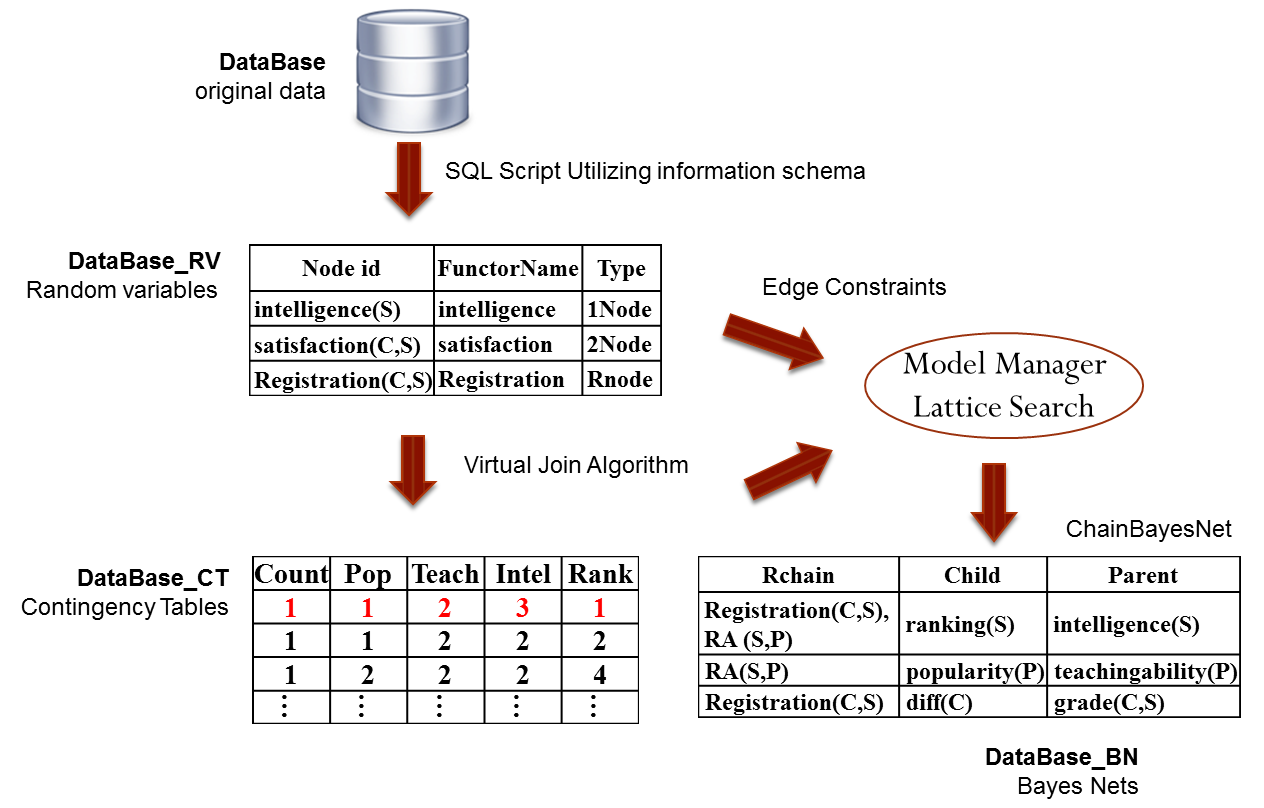
\includegraphics[width=0.8\textwidth]{figures/general-flow-chart.png}
%}
%\caption{Overview for the BayesBase system.
%%Here the $DB$ denotes the original database, $DB\_RV$ denotes the database storing all random variables, 
%%$DB\_CT$ denotes the database containing all the contingency tables  and $DB\_BN$ storing all the learned Bayes Nets.
%\label{fig:general-flow-chart}}
%\end{center}
%\end{figure}

\section{Background and Notation}
We adopt function-based notation from logic for combining statistical and relational concepts \cite{Russell2010,Poole2003,Getoor2006,Chiang2012}.

%\subsection{Relational Databases }
% \begin{table}[tbp] \centering
%\begin{tabular}
%[c]{|l|}\hline\\
%$\student$(\underline{$student\_id$}, $\intelligence$, $ranking$)\\
%$\course$(\underline{$course\_id$}, $\diff$, $rating$)\\ 
%$\prof$ (\underline{$professor\_id$}, $teaching\_ability$, $popularity$)\\
%$\reg$ (\underline{$student\_id$, $course\_id$}, $grade$, $satisfaction$)\\
%$\ra$ (\underline{$student\_id$, $prof\_id$}, $salary$, $capability$)\\
%$\it{Teaches} $(\underline{$professor\_id$, $course\_id$})\\
%\\
%\hline
%\end{tabular}
%\caption{Replace by a ER Diagram: A relational schema for a university domain. Key fields are underlined. An instance for this schema is given in Figure \ref{fig:university-tables}.
%\label{table:university-schema}} 
%\end{table}

\begin{figure}[htbp] %  figure placement: here, top, bottom, or page
 \centering
\resizebox{0.4\textwidth}{!}{
 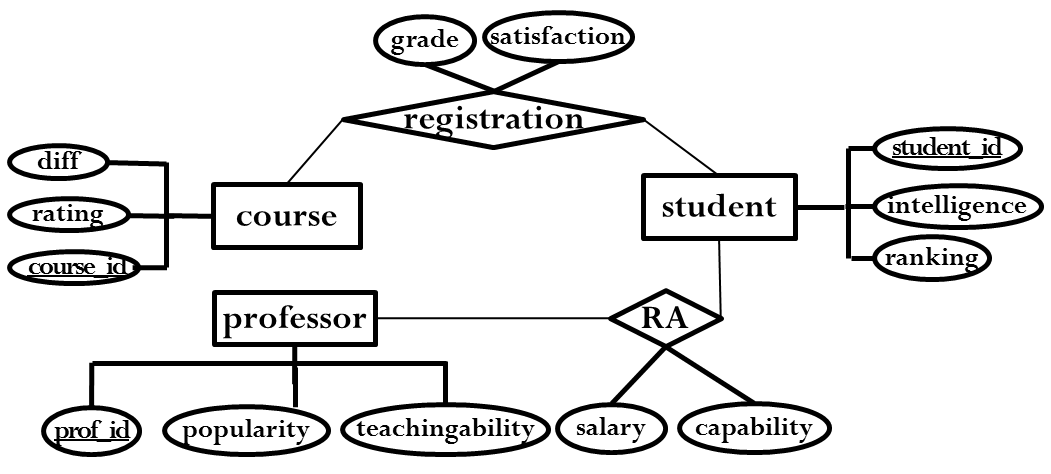
\includegraphics[width=0.5\textwidth]{figures/university-schema.png}
% 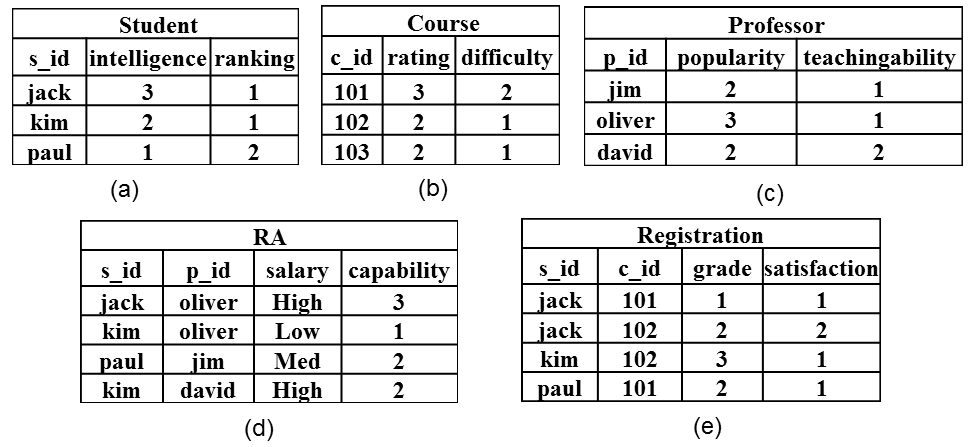
\includegraphics[width=0.5\textwidth]{figures/university-tables.png}  
} 
\caption{A relational ER Design for a university domain.}
 \label{fig:university-schema}
\end{figure}

 We assume a standard \textbf{relational schema} containing a set of tables, each with key fields, %typically
descriptive attributes, and possibly foreign key pointers. 
A \textbf{database instance} specifies the tuples contained in the tables of a given database schema. 
We assume that tables in the relational schema can be divided into {\em entity tables} and {\em relationship tables.} 
This is the case whenever a relational schema is derived from an entity-relationship model (ER model) \cite[Ch.2.2]{Ullman1982}. 
%The functor formalism is rich enough to represent the constraints of an ER schema by the following translation: Entity sets correspond to types, descriptive attributes to functions, relationship tables to predicates, and foreign key constraints to type constraints on the arguments of relationship predicates.  
%Assuming an ER design, a relational structure can be visualized as a complex network \cite[Ch.8.2.1]{Russell2010}: individuals are nodes, attributes of individuals are node labels, relationships correspond to (hyper)edges, and attributes of relationships are edge labels. Conversely, a complex  network can be represented using a relational database schema.


%Table \ref{table:university-schema} shows a relational schema for a database related to a university.
%In this example, there are three entity tables: a $\student$ table, a $\course$ table and a $\prof$ table.  
%The relationship table $\reg$ with foreign key pointers to the $\student$ and $\course$ tables whose tuples indicate which students have registered in which courses.
%
%The other two relationship tables have the similar foreign key constraints involving different entity tables. 
%
%Figure \ref{fig:university-tables} displays a small database instance for this schema together with a Parametrized Bayes Net (only considering the $\reg$ relationship for simplicity.) 
%%To keep the schema simple, we introduce only a limited number of attributes for each entity class. 
%
% 
%\begin{figure}[htbp] %  figure placement: here, top, bottom, or page
% \centering
%\resizebox{0.5\textwidth}{!}{
% 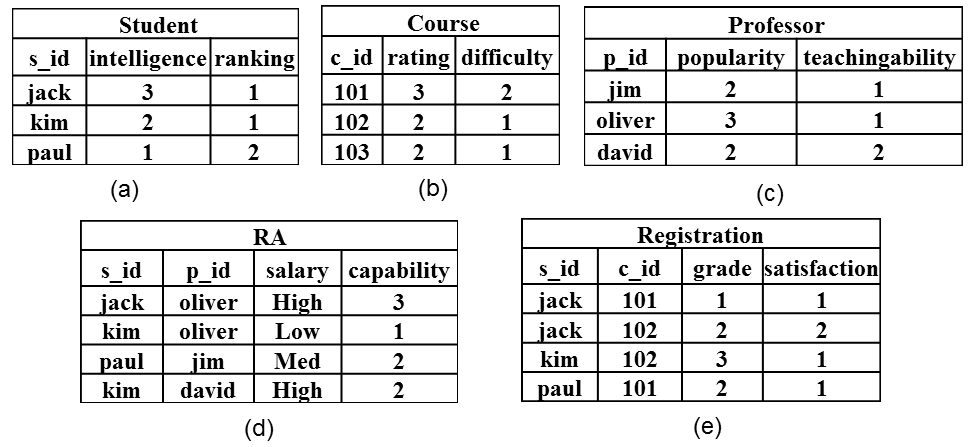
\includegraphics[width=0.5\textwidth]{figures/university-tables.png} 
%} 
%\caption{Database Table Instances: (a) $\student$, (b) $\course$, (c) $\reg$.  (d)A sample Parametrized Bayes Net based on the university schema.  % The $\cttable(\reg)$ table  is the contingency table for $\reg$ which we will introduce in Section~\ref {sec:mobius}. (e) 
%}
% \label{fig:university-tables}
%\end{figure}
%


%\subsection{Propositional Machine Learning}
%bla,bla,

\subsection{Relational Random Variables} %We adopt the PBN formalism, following Poole's presentation.
A domain or \textbf{population} is a set of individuals.
Individuals are denoted by lower case expressions (e.g., $\it{bob}$). 
%A \textbf{first-order variable} is capitalized. 
A \textbf{functor} represents a mapping
$\functor: \population_{1},\ldots,\population_{a} \rightarrow \outdomain_{\functor}$
where $\functor$ is the name of the functor, each $\population_{i}$ is a population, and $\outdomain_{\functor}$ is the output type or \textbf{range} of the functor. 
In this paper we consider only functors with a finite range, disjoint from all populations.  If $\outdomain_{\functor} = \{\true,\false\}$, the functor $\functor$ is a (Boolean) \textbf{predicate}. A predicate with more than one argument is called a \textbf{relationship}; other functors are called \textbf{attributes}. We use uppercase for predicates and lowercase for other functors.



%the populations associated with 
 %the variables are of the appropriate type for the functor.

A \textbf{Parametrized random variable} (PRV) is of the form $\functor(\X_{1},\ldots,\X_{a})$, where each $\X_{i}$ is a 1st-order variable. 
Each 1st-order variable is associated with a population that specifies its domain or type. 
We refer to the 1st-order variables as \textbf{first-order variables} to distinguish them from the parametrized random variables. %that appear in a Bayes net model. 


Figure \ref{fig:university-tables} displays a small database instance for this schema together with a Parametrized Bayes Net (only considering the $\ra$ relationship for simplicity.) 
%To keep the schema simple, we introduce only a limited number of attributes for each entity class. 

 
\begin{figure}[htbp] %  figure placement: here, top, bottom, or page
 \centering
\resizebox{0.4\textwidth}{!}{
 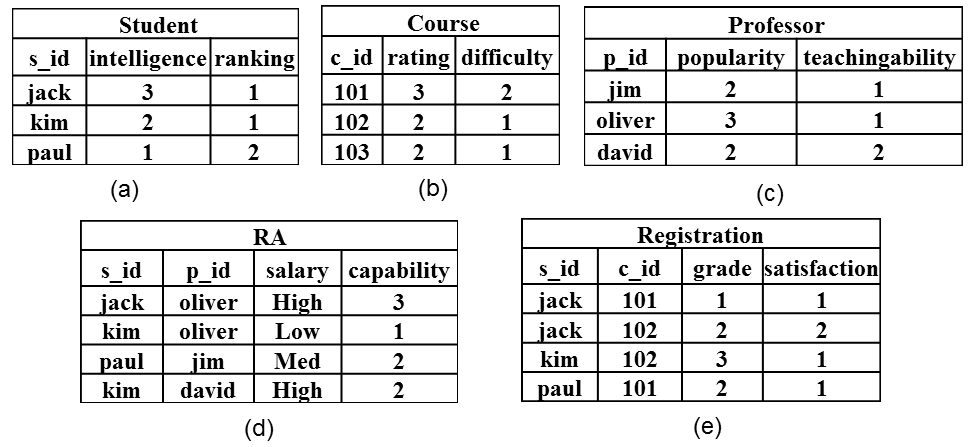
\includegraphics[width=0.5\textwidth]{figures/university-tables.png} 
} 
\caption{Database Table Instances.%: (a) $\student$, (b) $\prof$, (c) $\ra$.  (d) A sample Parametrized Bayes Net based on the university schema.  % The $\cttable(\reg)$ table  is the contingency table for $\reg$ which we will introduce in Section~\ref {sec:mobius}. (e) 
}
 \label{fig:university-tables}
\end{figure}



\subsection{Contingency Tables}
%Our starting point is the observation that a statistical learning algorithm like a Bayes net learner does not require an enumeration of individuals tuples, but only {\em sufficient statistics} \cite{Heckerman1995,Schulte2011}. 
%It is well-known in machine learning that a statistical learning algorithm like a Bayes net learner does not require an enumeration of individuals tuples, but only {\em sufficient statistics} \cite{Heckerman1995,Schulte2011}. 
Sufficient statistics can be represented in {\em contingency tables} as follows \cite{Moore1998}. 
%
 %A contingency table is defined as follows.
%The Bayes net is learned from the contingency table. 
%
%The count column in the $\ct$-table represents the number of instantiations for a given tuples of values in a row in the input database. 
%
Consider a fixed list of  random variables.
%$\R_{1}, R_{2},\ldots,R_{m}$, and attribute nodes $\functor_{1},\ldots,\functor_{j}$. 
A \textbf{query} is a set of $(variable = value)$ pairs where each value is of a valid type for the random variable. 
The \textbf{result set} of a query in a database $\D$ is the set of instantiations of the first-order variables such that the query evaluates as true in $\D$.
For example, in the database of Figure~\ref{fig:university-tables} the result set for the query 
%$(\it{intelligence}(\S) = 2$, $\it{rank}(\S) = 1$, $\it{rating}(\C) = 3$, $\it{diff}(\C) = 1$, $\reg(\S,\C) = F)$
$(\it{intelligence}(\S) = 2$, $\it{rank}(\S) = 1$, $\it{popularity}(\P) = 3$, $\it{teachingability}(\P) = 1$, $\ra(\P,\S) = T)$ is the singleton $\{\langle \it{kim}, \it{Oliver}\rangle\}$. 
% $\{\langle \it{kim}, \it{101}\rangle\}$
The \textbf{count} of a query is the cardinality of its result set. 

Every set of variables $\set{V} = \{\V_{1}$,$\ldots,\V_{n} \}$ has an associated \textbf{contingency table} denotes by $\ct(\set{V})$. %$CT(\set{V})$. 
This is a table with a row for each of the possible assignments of values to the variables in $\set{V}$, and a special integer column called $\qcount$. 
The value of the $\qcount$ column in a row 
corresponding to $V_{1} = v_{1},\ldots,V_{n} = v_{n}$ records the count of the 
corresponding query. 
Figure~\ref{fig:ct} shows the contingency table from university database. 
The value of a relationship attribute is undefined for entities that are not related.
Following \cite{Milch2007}, %\cite{BLOG}, 
%$\it{capability(\P,\S)} = n/a $
we indicate this by writing 
%$\it{grade}(\s,\c) = n/a$ 
$\it{capability(\P,\S)} = n/a $ for a reserved constant $\it{n/a}$. 
The assertion $\it{capability(\P,\S)}$ = n/a is therefore equivalent to the assertion that $\ra(\P,\S) = \false$.
%For example, if student $\s$ is not registered in course $\c$, the value of $\it{grade}(\s,\c)$ is undefined. 


\begin{figure}[htbp]
\begin{center}
\resizebox{0.4\textwidth}{!}{
%%!%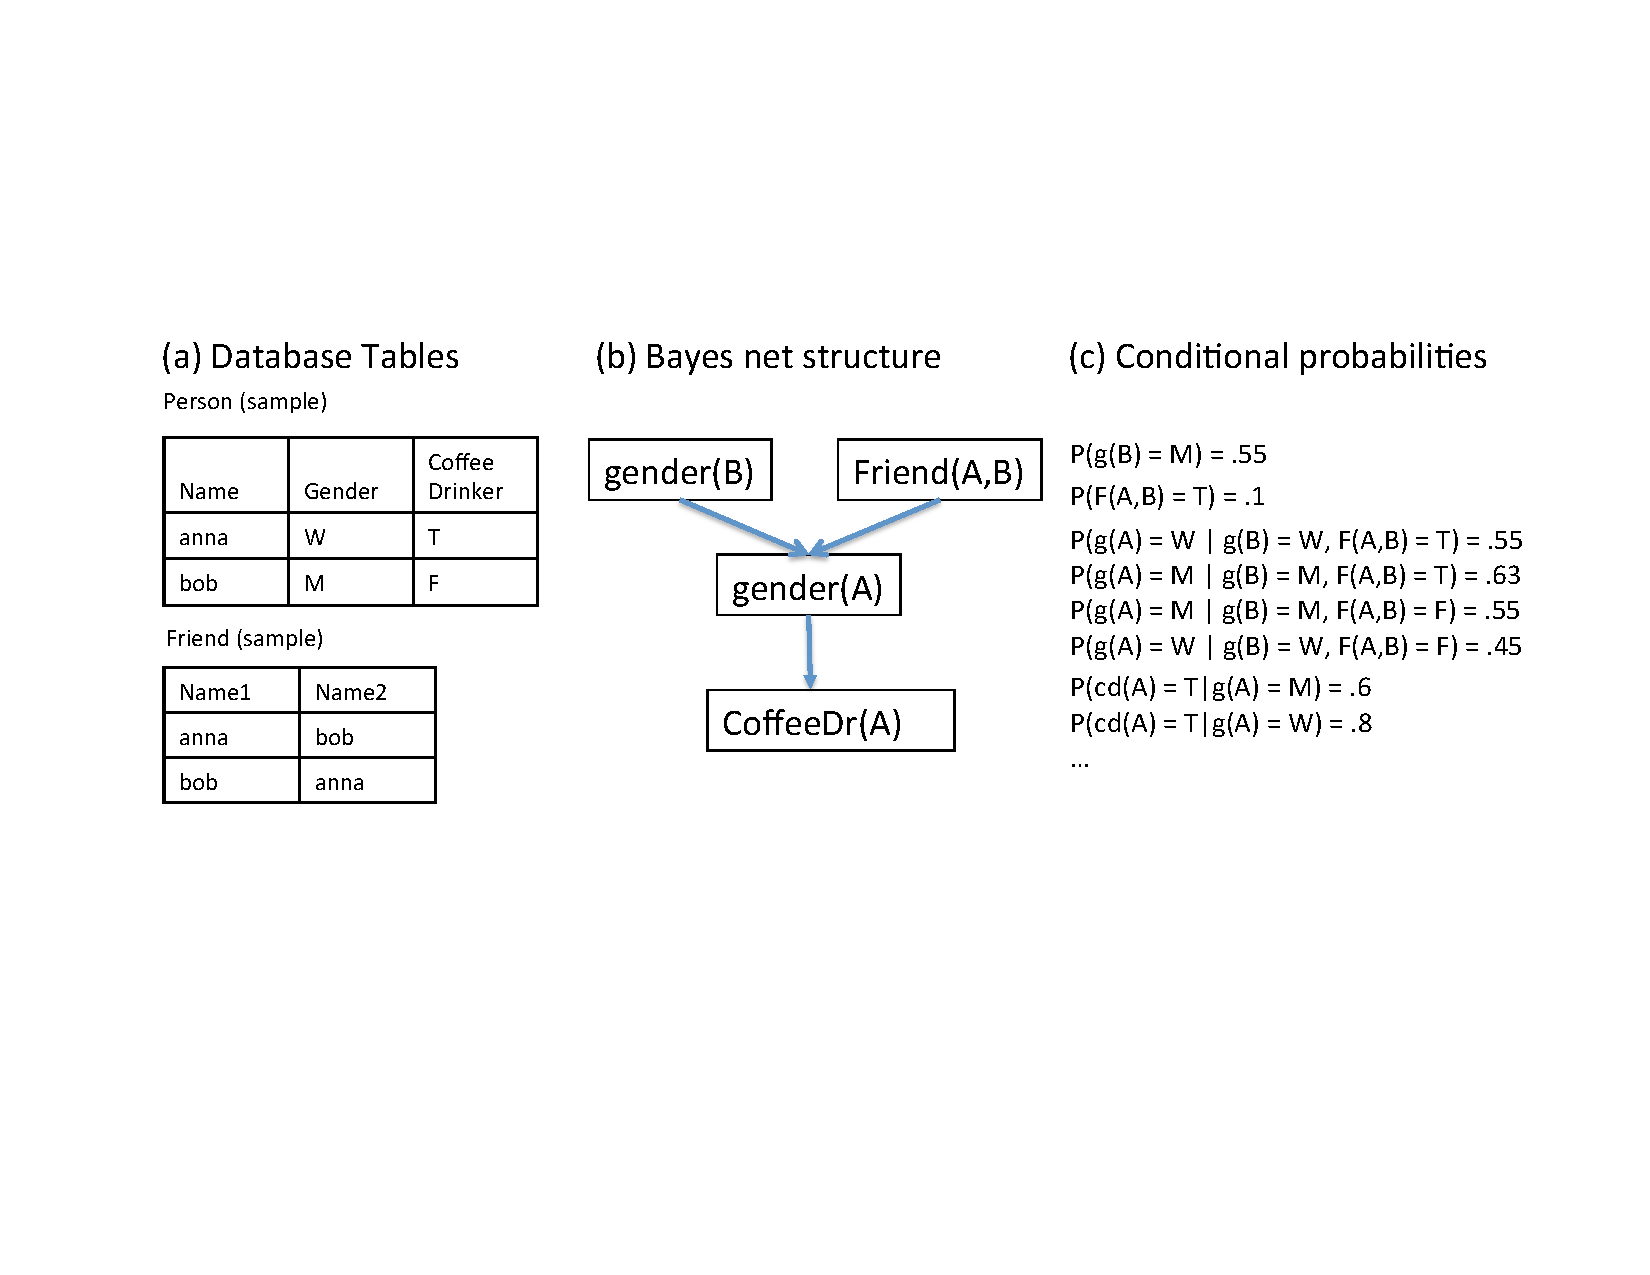
\includegraphics[width=1\textwidth]{pbn}
%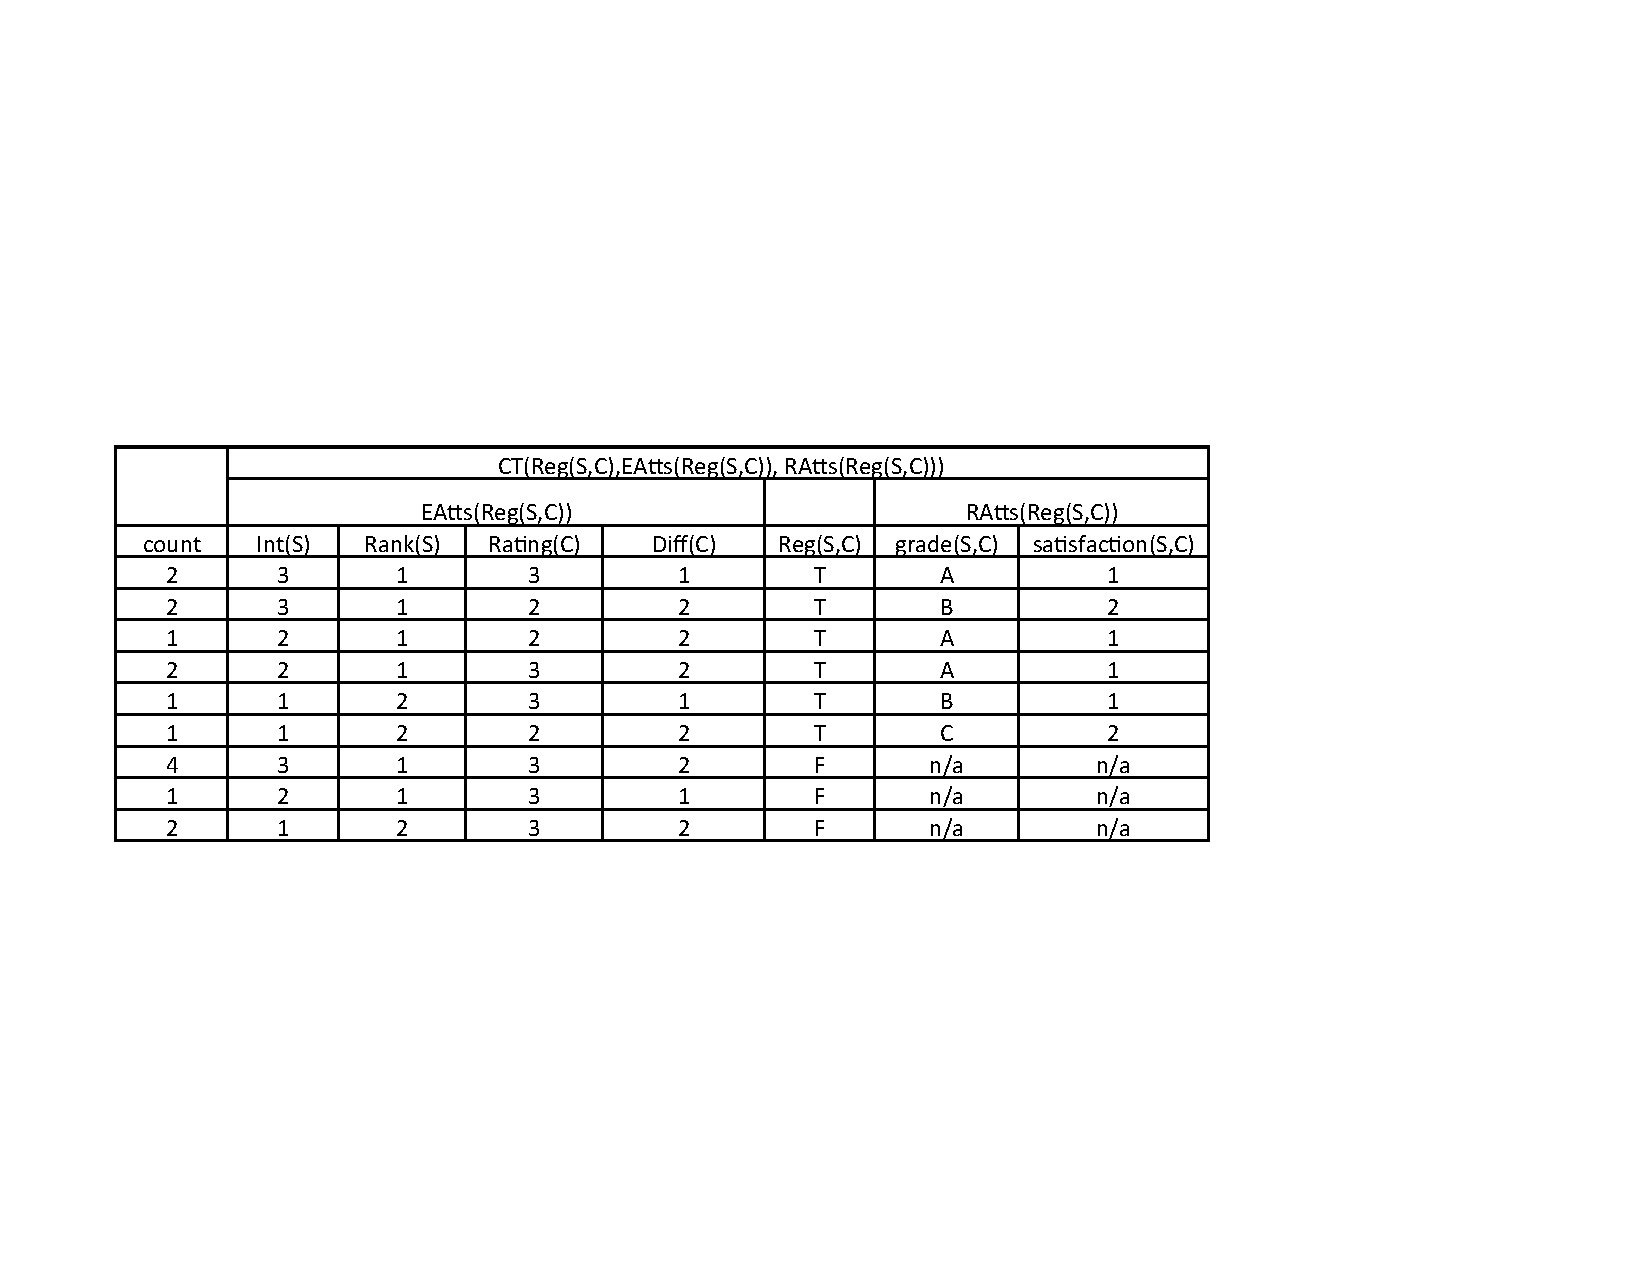
\includegraphics{figures/ct-table.pdf}
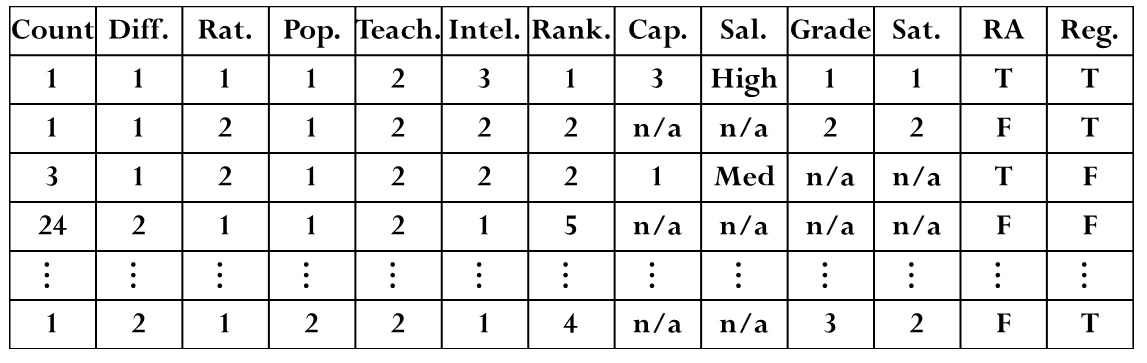
\includegraphics[width=0.5\textwidth]{figures/uni-ct-table.JPG}
}
\caption{Excerpt from the joint contingency table for the university database of Figure~\ref{fig:university-tables}. % for the attribute-relation table of Figure~\ref{fig:university-tables}
Each row shows a query and its instantiation count in the database.
%one possible assignment of such nodes with its count. 
% where for illustration we have added counts for another student like Jack and another course like 103.
%use partial real table
\label{fig:ct}}
\end{center}
\end{figure}

A \textbf{conditional contingency table}, written $$\ct(V_{1},\ldots,V_{k}|V_{k+1} = v_{k+1},\ldots, V_{k+m} = v_{k+m})$$
is the contingency table whose column headers are $V_{1},\ldots,V_{k}$ and whose counts are  defined by subset of instantiations that match the condition to the right of the $\vert$ symbol.  %  \textbar 
For compactness, our algorithms work with contigency tables that omit rows with count 0.

\subsection{Bayes Nets for Relational Data}

Poole introduced the Parametrized Bayes net (PBN) formalism that combines Bayes nets with logical syntax for expressing relational concepts \cite{Poole2003}. A {\bf Bayes Net (BN)} is a directed acyclic graph (DAG) whose nodes comprise a set of random variables and conditional probability parameters.
For each assignment of values to the nodes, the joint probability 
is specified by the product of the conditional probabilities, $P(\it{child}|\it{parent\_values}$). A \textbf{Parametrized Bayes Net} (PBN) is a Bayes net whose nodes are Parametrized random variables \cite{Poole2003}. 
Since in our machine learning application, Parametrized random variables appears in Bayes net, we often refer to them simply as \textbf{nodes}. Figure \ref{fig:bn-example} shows a PBN for the University database.

\begin{figure}[htbp] %  figure placement: here, top, bottom, or page
 \centering
\resizebox{0.3\textwidth}{!}{
 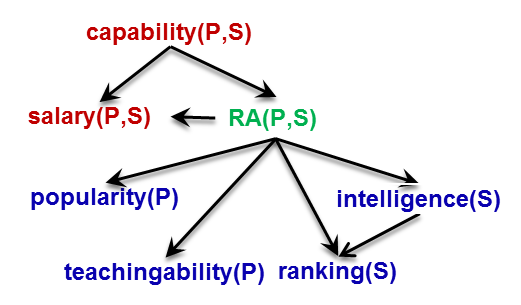
\includegraphics[width=0.3\textwidth]{figures/bn-example.png} 
} 
\caption{ A sample Parametrized Bayes Net based on the university schema. 
}
 \label{fig:bn-example}
\end{figure}


\section{Specification of Parametrized Random Variables}

The Virtual Join algorithm takes as input a relational database and a set of parametrized random variables or nodes and returns a contingency table for the set. In this section we discuss how to represent a set of PRVs.
%Bayes net nodes.
%parametrized random variables. 
%This set can be defined by the user, or generated based on the database schema information. 


%We define a default set of parameterized random variables for  a target relational database. 
%We show that this set and metainformation about the random variables can be computed from the database system catalog. % using SQL queries. 
\subsection{The Random Variable Database}
The information about the random variables is stored in the \textbf{random variable database}.  
%This database provides metainformation for machine learning analysis analogous to the way in which the system catalog provides metainformation for database queries. The definitions of the random variables are stored in tables in the random variable database, together with useful metainformation about the random variables, such as their domains and the sizes of their domains. 
%
The Virtual Join algorithm distinguishes three types of PRVs, 1Nodes, RNodes, and 2Nodes. 
For each attribute of an entity, there is a corresponding attribute node called a \textbf{1Node} for short. The domain of a 1Node is the same as that of the corresponding attribute.  There is a Boolean random variable for each relationship set, called a \textbf{relationship node} or \textbf{RNode} for short.
Throughout this paper we assume that all relationships are binary, though this is not essential for our algorithm. 
For each attribute of an relationship, there is a corresponding attribute node called a \textbf{2Node} for short. The domain of a 2Node is the same as that of the corresponding attribute. 
%In logical terms, nodes are interpreted as functions that return a value for a given input entity tuple \cite{Milch2007}.
Table~\ref{table:translation} illustrates %the mapping from the ER design to 
the logical functor notation and its relationship to the database ER diagram. 

%
%The basic set of random variables is derived from the elements of an ER design.
%Table~\ref{table:translation} illustrates the mapping from the ER design to the logical functor notation. 
%There is a random variable for each entity set, called a \textbf{first-order variable}. 
%The domain of first-order variables comprises the entities in the associated entity set. 
%There is a Boolean random variable for each relationship set, called a \textbf{relationship node} or \textbf{RNode} for short.
%Throughout this paper we assume that all relationships are binary, though this is not essential for our system. 
%For each attribute of an entity, there is a corresponding attribute node called a \textbf{1Node} for short. The domain of a 1Node is the same as that of the corresponding attribute.  
%For each attribute of an relationship, there is a corresponding attribute node called a \textbf{2Node} for short. The domain of a 2Node is the same as that of the corresponding attribute. 
%In logical terms, nodes are interpreted as functions that return a value for a given input entity tuple \cite{Milch2007}.
%As the table shows, we refer to the attributes of a first-order variable $\A$ collectively as $1Nodes(\A)$ and to the attributes of a relationship node $\R$ collectively as $2Nodes(\R)$. %\cite{BLOG}. 

%The value of a relationship attribute is undefined for entities that are not related.
% For example, if student $\s$ is not registered in course $\c$, the value of $\it{grade}(\s,\c)$ is undefined. 
%Following \cite{Milch2007}, 
%%\cite{BLOG}, 
%we indicate this by writing $\it{grade}(\s,\c) = n/a$ for a reserved constant $\it{n/a}$. 
%The assertion $\it{grade}(\s,\c) = n/a$ is therefore equivalent to the assertion that $\reg(\s,\c) = \false$.
 



%\begin{figure}[htbp]
%\begin{center}
%\resizebox{0.5\textwidth}{!}{
%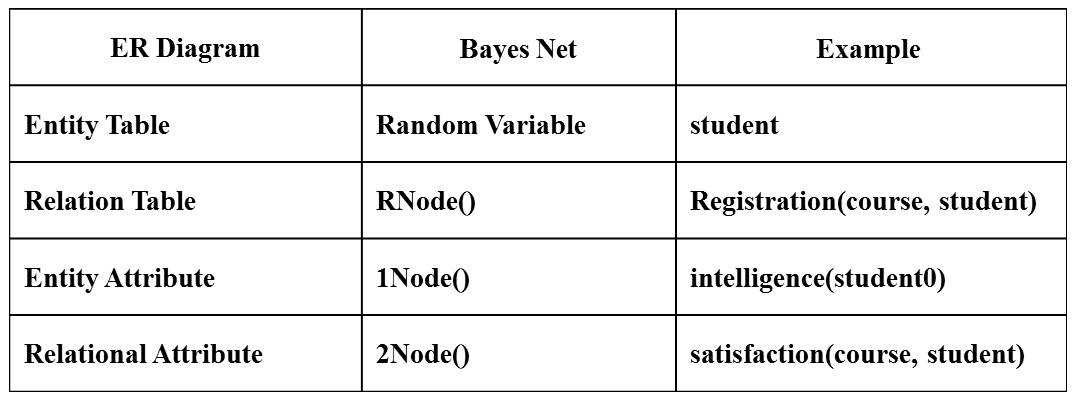
\includegraphics[width=0.5\textwidth]{figures/translation.png}
%}
%\caption{Translation from ER Diagram of Relational Database to Bayes Nets.
%\label{fig:translation}}
%\end{center}
%\end{figure}

%\begin{table}[btp] \centering
%\resizebox{0.5\textwidth}{!}{
%\begin{tabular}[c]
%{|l|l|l|l|}\hline
% ER Design &Bayes Net & Example &Term Notation\\\hline
%    Entity Tables&Population Variables  & Student, Course & S, C \\\hline
%    Relation Tables &RNodes &Registration & Registration(C,S) \\\hline
%   Entity Attributes &1Nodes & intelligence, ranking & \{intelligence(S), ranking(S)\} = 1Nodes(S) \\\hline
%   Relationship Attributes &2Nodes & satisfaction, grade & \{satisfaction(C, S), grade(C,S)\} = 2Nodes(Registration(C,S)) \\\hline
%   
%\end{tabular}
%}
% % end scalebox
%\caption{Translation from ER Design of Relational Database to Bayes Nets.
% \label{table:translation}}
%\end{table}
\begin{table}[btp] \centering
\resizebox{0.4\textwidth}{!}{
\begin{tabular}[c]
{|l|c|l|l|}\hline
  \begin{tabular}{l}ER \\Design \end{tabular}&Type & Functor &PRV \\\hline
   % \begin{tabular}{l}Entity \\Tables\end{tabular}&\begin{tabular}{l}Population \\Variables \end{tabular} & Student, Course & S, C \\\hline
    \begin{tabular}{l}Relation \\Tables \end{tabular}&RNodes &RA & RA(P,S) \\\hline
   \begin{tabular}{l}Entity \\Attributes \end{tabular}&1Nodes & intelligence, ranking &\begin{tabular}{l} \{intelligence(S), ranking(S)\}  \\=1Nodes(S) \end{tabular} \\\hline
  \begin{tabular}{l} Relationship \\Attributes \end{tabular}&2Nodes & teachingability, salary &\begin{tabular}{l}   \{teachingability(P,S), salary(P,S)\}  \\= 2Nodes(RA(P,S))\end{tabular}\\\hline
   
\end{tabular}
}
 % end scalebox
\caption{Translation from ER Diagram to Parametrized Random Variables. Population variables are derived from entity tables as described in the text.
 \label{table:translation}}
\end{table}

%{\em Database Representation.} 
The definitions of the three types of PRVs are listed in three tables in the
 Random Variable Database. 
This database also provides information about the random variables that is required for learning, such as their domains and the sizes of their domains. We refer to this information about the random variables for analysis as \textbf{metainformation}. 
%Utilizing the metainformation allows us to develop general schema-independent learning algorithms. 

\subsection{Generating Default PRVs} Defining a set of PRVs for a given database requires some user expertise in translating domain knowledge into the functor representation and metainformation.
% terms of understanding the functor representation and extracting metainformation. 
An alternative is to exploit the database schema catalog to generate default random variable database.
We use this default in the experiments reported below.  Because the system metadata is always available for any relational database,  by exploiting it, default random variables can be generated in a completely general way. This means that the Random Variable Database can be set up with no information from the user beyond  the SQL system catalog. However, the user does have the option to change the random variable metainformation, by editing the tables in the Random Variable Database.


Given an ER-diagram, it is straightforward to generate functors as illustrated in Table~\ref{table:translation}.
 Given a database information schema, we can compute an implicit ER diagram by reversing the standard translation from ER-diagrams to SQL \cite{Ullman1982}.
For instance, if a table contains a single primary key column and no foreign key pointers, we treat it as representing an entity set and associate a first-order variable with it. 
Since the database information schema is itself stored in table form, the default random variable database can be created using an SQL script. 
We omit further details due to space constraints.

The main complication arises when the database contains a self-relationship \cite{Heckermann} that relates two entities of the same type. If the schema contains a self-relationship, we add one first-order variable for each role in the relationship, and one set of 1Nodes for each first-order variable. 
%, when we need to introduce more than one relationship node for the relationship functor. 
For example, the Mondial database contains a self-relationship $\it{Borders}$ that relates two countries. 
%In the ER diagram, there are two lines from the $\it{Countries}$ entity set to the $\it{Borders}$ relationship set 
%The ring structure may be represented with two different first-order variables that each refer to the $\it{Countries}$ entity set. 
The corresponding relationship node is $\it{Borders}(\C_{1},\C_{2})$ . The different positions of the first-order variables can represent different roles in the self-relationship.
 In the Mondial example, there are two 1Nodes $\it{continent}(\C_{1})$ and $\it{continent}(\C_{2})$.


%To build a table with definitions of nodes, we represent a node as a tuple of the form $\langle \functor, \it{pv}_1, \ldots, \it{pv}_\ell \rangle$; in this paper we assume that  $\ell = 1,2$. Table~\ref{table:translation} shows examples.
%Adding first-order variables to functors generally requires only utilizing the primary key information to find which entities are associated with each functor and then using the first-order variables constructed in the previous step. If we find a self-relationship, we add one first-order variable for each role in the relationship, and one set of 1Nodes for each first-order variable. 
%
%We first discuss computing a default set of first-order variables and functors from the schema information, then combining the variables with the functors to form terms.
%
%\begin{algorithm}[htbp]
%\caption{Generating a default set of functors for modelling a target database. Can be implemented with SQL queries to the database information schema.}
%\label{alg:functors}
%%\linesnumbered
%\SetKwData{KwCalls}{Calls}
%\SetKwData{KwCondition}{Precondition:}
%\KwIn{Database Information Schema; Target Database $\D$}
%\KwOut{Tables with meta information about functors, stored in the random variable database $\D_{\RV}$.}
%\begin{algorithmic}[1]
%\STATE Find tables in $\D$ with a single primary key field. Store table names in $\D_{\RV}.\it{EntityTables}$.
%\STATE For each entity table, %.
%add one first-order variable entry $(\it{pv})$ in $\D_{\RV}.\it{Pvariables}$.
%\STATE For each entity table, for each column that is not part of the primary key, add an entry $(\it{column\_name})$ in $\D_{\RV}.\it{1Functors}$.
%%\STATE For each entity table, for each column that is not part of the primary key, add an entry $(\it{column\_name},\it{pv})$ in $\D_{\RV}.\it{1Functors}$.
%\STATE Find tables in $\D$ with two primary key columns that reference entity tables. Store table names in $\D_{\RV}.\it{RelationTables}$.
%% \STATE For each relation table, add an entry $(\it{table\_name}, \it{pv}_{1}, \it{pv}_{2})$ to $\D_{\RV}.
% \STATE For each relation table, add an entry $(\it{table\_name})$ to $\D_{\RV}
%\it{RFunctors}$. 
%\STATE For each relation table , for each column that is not part of the primary key, add an entry $(\it{column\_name})$  in $\D_{\RV}.\it{2Functors}$.
%%\STATE For each relation table , for each column that is not part of the primary key, add an entry $(\it{column\_name}, \it{pv}_{1}, \it{pv}_{2})$  in $\D_{\RV}.\it{2Functors}$.
%\end{algorithmic}
%\end{algorithm}
%
%
%\subsection{Generating Nodes}
%There are many statistical dependencies that functors by themselves are not sufficient to express. 
%These concern relational autocorrelations \cite{jensen}, where the attribute values of related entities influence each other. This type of dependency occurs when the ER diagram contains a self-relationship.
%%, when we need to introduce more than one relationship node for the relationship functor. 
%For example, the Mondial database contains a self-relationship $\it{Borders}$ that relates two countries. In the ER diagram, there are two lines from the $\it{Countries}$ entity set to the $\it{Borders}$ relationship set that form a ring \cite{ullmann}. \textbf{role in relationship? ring?}
%The ring structure may be represented with two different first-order variables that each refer to the $\it{Countries}$ entity set. The corresponding relationship node is $\it{Borders}(\C_{1},\C_{2})$ . The different positions of the variables can represent different roles in the relationship. 
%%Since we introduce two first-order variables referring to the same entity set, we need to duplicate the 1Nodes for that entity set. 
%This allows the logical language to represent that attributes of neighboring countries influence each other, 
%%Using a second relationship node with the $\it{Borders}$ functor allows us to represent such influences, 
%for instance in the following rule
%$$\it{continent}(\C_{1}) = \it{Europe}, \it{Borders}(\C_{1}, \C_{2}) = \true \rightarrow \it{continent}(\C_{2}).$$
%
%To build a table with definitions of nodes, we represent a node as a tuple of the form $\langle \functor, \it{pv}_1, \ldots, \it{pv}_\ell \rangle$; in this paper we assume that  $\ell = 1,2$. Table~\ref{table:translation} shows examples.
%Adding first-order variables to functors generally requires only utilizing the primary key information to find which entities are associated with each functor and then using the first-order variables constructed in the previous step. If we find a self-relationship, we add one first-order variable for each role in the relationship, and one set of 1Nodes for each first-order variable. 
%-unielwin: pvariable, rnodes,1nodes, 2nodes.... show the whole setup database.
%- Pseudocode for explaining the metadata script. in Figure \ref{fig:rv_db}
%- mention self-relationship detail
%
%
%\begin{figure}[htbp]
%\begin{center}
%\resizebox{0.5\textwidth}{!}{
%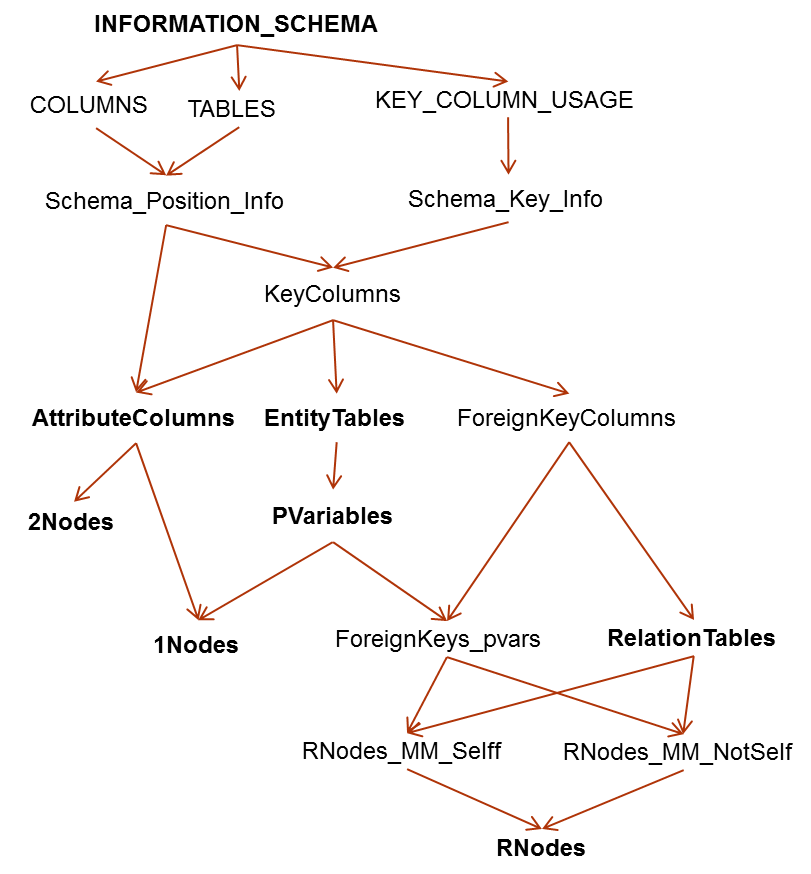
\includegraphics[width=0.5\textwidth]{figures/rv_db.png}
%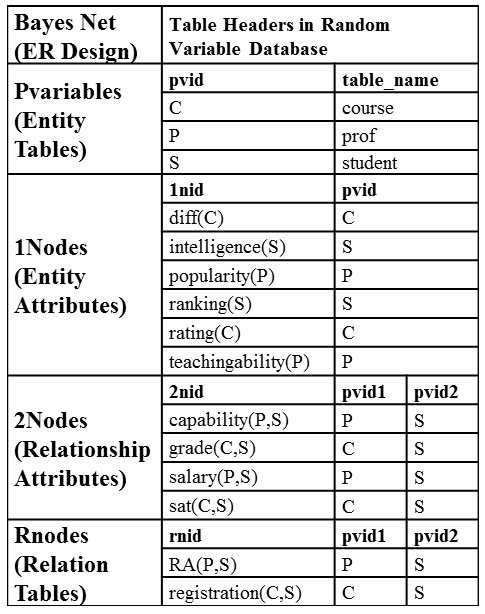
\includegraphics[width=0.5\textwidth]{figures/rv_db_tables.png}
%}
%\caption{Flow chart for Random Variable Database.
%\label{fig:rv_db}}
%\end{center}
%\end{figure}

\section{Relational  Contingency Tables}
%Relational learning algorithms explore longer and longer chains of relationships that may link statistically dependent objects. 
Many relational learning algorithms take an iterative deepening approach [cite jensen]: explore correlations along paths defined by single links, then along paths defined by a link chain of length 2, 3, etc. 
Chains of relationships form a natural lattice structure. In terms of this lattice, iterative deepening corresponds to moving from the bottom to the top. 
%
%Conceptually, the lattice view simplifies describing and developing learning algorithms. Computationally, 
The Virtual Join algorithm computes contingency tables by using the results for smaller relationships for larger relationship chains, which leads to an efficient dynamic program. Another benefit of level-wise lattice learning is that if the learning algorithm requires sufficient statistics only up to a certain depth in the lattice, the Virtual Join algorithm can be restricted to this depth. %The lattice diagram facilitates the computation of contingency tables that summarize the sufficient database statistics for learning.
%
%\subsection{The Relationship Lattice}
%

A relationship set is a \textbf{chain} if it can be ordered as a list $[\Relation_{1}(\argterms_{1}),\ldots,\Relation_{k}(\argterms_{k})]$ 
%is a \textbf{chain} if 
such that each functor $\Relation_{i+1}(\argterms_{i+1})$ shares at least one first-order variable with the preceding terms $\Relation_{1}(\argterms_{1}),\ldots,\Relation_{i}(\argterms_{i})$.
%\footnote{Essentially the same concept is called a slot chain in PRM modelling \cite{Getoor2007c}.}
%A relationship set forms a chain if the corresponding list is a chain. 
All sets in the lattice are constrained to form a chain.
%
For instance, in the University schema of Figure~\ref{fig:university-schema}, a %relationship 
chain is formed by the two relationship nodes
\[\reg(\S,\C),\ra(\P,\S).\]
%list \[[\it{RA}(\P,\S),\it{Registered}(\S,\C)].\] 
If relationship node $\it{Teaches}(\P,\C)$ is added,
%to record which student is a TA for which course,
we may have a three-element chain \[\reg(\S,\C),\ra(\P,\S),\it{Teaches}(\P,\C).\] 
The subset relation defines a lattice on relationship sets/chains. 
Figure~\ref{fig:big-lattice} illustrates the  lattice for the relationship nodes in the university schema. 
For reasons that we explain below, entity tables are also included in the lattice and linked to relationships that involve the entity in question. 

\begin{figure}[htbp]
\begin{center}
\resizebox{0.5\textwidth}{!}{
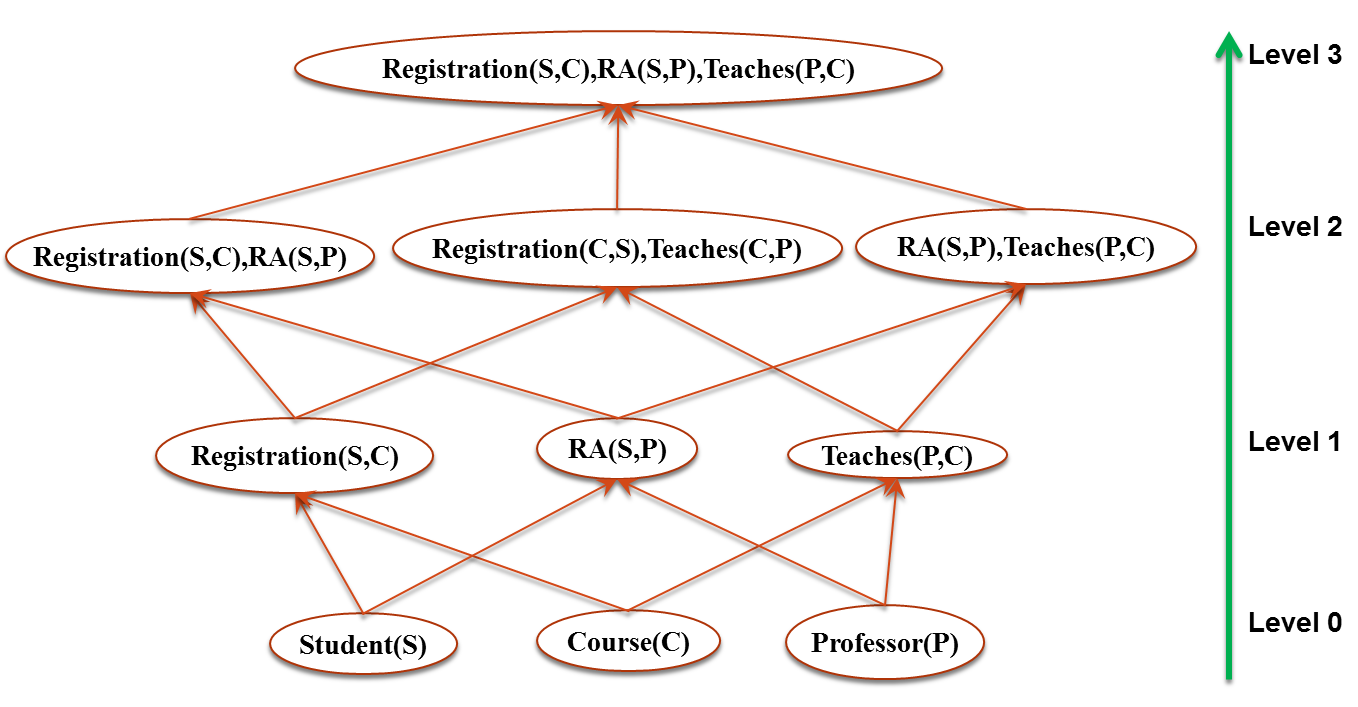
\includegraphics[width=0.8\textwidth]{figures/uni-big-lattice.png}
}
\caption{A lattice of relationship sets for the university schema of Figure~\ref{fig:university-schema}.
 Links from entity tables to relationship tables correspond to foreign key pointers. 
%The list representation of the sets is determined by the functor ordering $\it{Registered} < \it{TA} < \it{Teaches}$. 
\label{fig:big-lattice}}
\end{center}
\end{figure}




With each relationship chain $\set{\Relation}$ is associated a $\ct$-table $\ct_{\set{\Relation}}$. 
For a relationship chain $\set{\Relation}$ the nodes in the $\ct$-table  $\ct_{\set{\Relation}}$%$\B_{\set{Relation}}$
 comprise: the Rnodes in the set $\set{\Relation}$, the 1Nodes and 2Nodes associated with each of the Rnodes. To describe these, we introduce the following notation.
%Let's first introduce the notations for all kinds of functor nodes in order to extend relational algebra operators for manipulating $\qcount$ in contingency tables as follows.
%Let $R$ be a relationship node and let $\set{R}$ be a set of relationship nodes.

\begin{itemize}
\item $\eatts(R)$ denotes the set of entity attribute nodes for the first-order variables involved in the relationship $R$. 
\item $\eatts(\set{R})$ is the union of the entity attributes for each relationship $R \in \set{R}$.
\item $\ratts(R)$ denotes the set of relationship attribute nodes for %the first-order variables involved in 
the relationship $R$.
\item $\ratts(\set{R})$ is the union of the relationship attributes for each relationship $R \in \set{R}$.
\item $\atts(R)$ is the set of both entity and relationship attributes for relationship $R$, similarly for $\atts({\set{R}})$.
\item  $1Nodes(\A)$ denotes the attributes of a first-order variable $\A$ collectively
%\item $R_{i}$ is the Boolean relationship node.
%\item $\etable$ denotes a entity table.
%\item $Column\_List({\etable})$ is the set of non-count columns in entity table $\etable$.
\end{itemize}

In this notation, the nodes in the $\ct$-table  $\ct_{\set{\Relation}}$  are denoted as $\set{\Relation} \cup \atts({\set{R}})$. 

\emph{Implementation.} The Random Variable Database specifies the set of relationship nodes for building the lattice. Building a lattice of relationship chains can be done using any standard technique, such as those developed for enumerating itemsets in association rule  mining \cite{Agrawal1994}. 
We create a table {\em Lattice} in the Bayes net database with one row for each relationship chain. We also create two auxilliary tables: One that lists which relationship chains are children of which others. A child contains exactly one more relationship node (cf. Figure~\ref{fig:big-lattice}). 
%For example, the relationship chain $\it{Registration}(\S,\C),\it{RA}(\S,\P)$ is a child of the chain $\it{Registration}(\S,\C)$. Another auxilliary table lists which relationship nodes are members of which relationship chain. For example, the relationship chain $\it{Registration}(\S,\C),\it{RA}(\S,\P)$ has two members. The auxilliary tables are used during learning as described below.

The goal of the Virtual Join Algorithm is to compute a contingency table for each point in the lattice. 
In the example of Figure~\ref{fig:big-lattice}, the algorithm computes 10 contingency tables. The $\ct$-table for the top element of the lattice is the \textbf{joint $\ct$-table} for the entire database. 
It is useful to distinguish two types of rows within each $\ct$-table: rows where all the relationship nodes are assigned the value $\true$---positive relationships only---and rows where one or more relationship nodes are assigned the value $\false$---some negative relationships. 
We begin with the case of positive relationships only.


%\section{Computing Relational Contingency Tables} \label{sec:cta}
\section{Computing Contingency Tables For Positive Relationships} 


%The learning algorithms described in this paper rely on the  availability of the $\ct$-tables (see Figure~\ref{fig:university-tables}). 
%Computing the contingence tables raises two key challenges that we address in this paper. 
If a conjunctive query involves only positive relationships, then it can be computed using SQL's sum aggregate function applied to a table join. The SQL sum query represents the positive part of the $\ct$-table much like a view definition represents a relation. 
To achieve a general solution without advance knowledge of the database schema, we need to construct the SQL sum query from metainformation. 
We propose accomplishing this via a \textbf{metaquery}.
%: Using the meta-information in the random variable database, we construct an SQL query for each relationship chain. 
%The SQL query represents a table join followed by a sum aggregation. Executing this query constructs the positive relationship part of the contingency table. 

%In the next section we proposed a new approach for the second challenge.
%
%The second challenge is computing event counts that involve negative relationships. This is infeasible using standard table joins [explain: firends vs un-firends]. 
%We approach this problem in two steps. 
%First, we show that event counts using $m+1$ negative relationships can be computed from two event counts that each involve at most $m$ relationships. 
%We state this result as a relational algebra identity in a new extension of relational algebra that we term \textbf{contingency table algebra}. A dynamic programming algorithm applies the algebraic identify repeatedly to efficiently build up a complete contingency table from partial tables that involve fewer negative relationships. 
%
%\subsection{Metaqueries for Utilizing Schema Information} 
%%As the top level of  Figure~\ref{fig:flow} illustrates, 
%The required counts involving only true relationships can be computed using the standard SQL constructs COUNT(*) and GROUP BY. 
%The general form of these operations is the same for every input database. 
%The varying part is the list of columns to be included, which depends on the input database. 
%For a fixed database, the column lists can be hard-coded. 
%To achieve a general solution when the column list is not known in advance, we introduce a new approach that we refer to as an SQL \textbf{meta query}. 
%
An SQL meta query is an SQL query that takes as input schema information as recorded in the random variable database,
and produces four kinds of tables: the Select, From, Where and Group By tables. The Select table lists the entries in the Select clause of the target query, the From table lists the entries in the From clause, and similar for Where and GROUP BY tables. %\footnote{basically the Group BY table is same as Select table without $\qcount$ column}. 
%Thus an SQL meta query maps schema information to the components of another SQL query. 
Given the four query tables, the corresponding SQL query can be easily executed in an application or stored procedure to produce the $\ct$-table entries.
Figure~\ref{fig:meta-query} shows an example of metaqueries for the university database. The metaquery accesses tables in the Random Variable Database $RV$. The entries of the Group By table (not shown) are the same as the Select table without the $\qcount$ column.
The $\it{@database@}$ is a string placeholder for the input database name. We omit further details due to space constraints.

\begin{figure}[htb]
\begin{center}
\resizebox{0.5\textwidth}{!}{
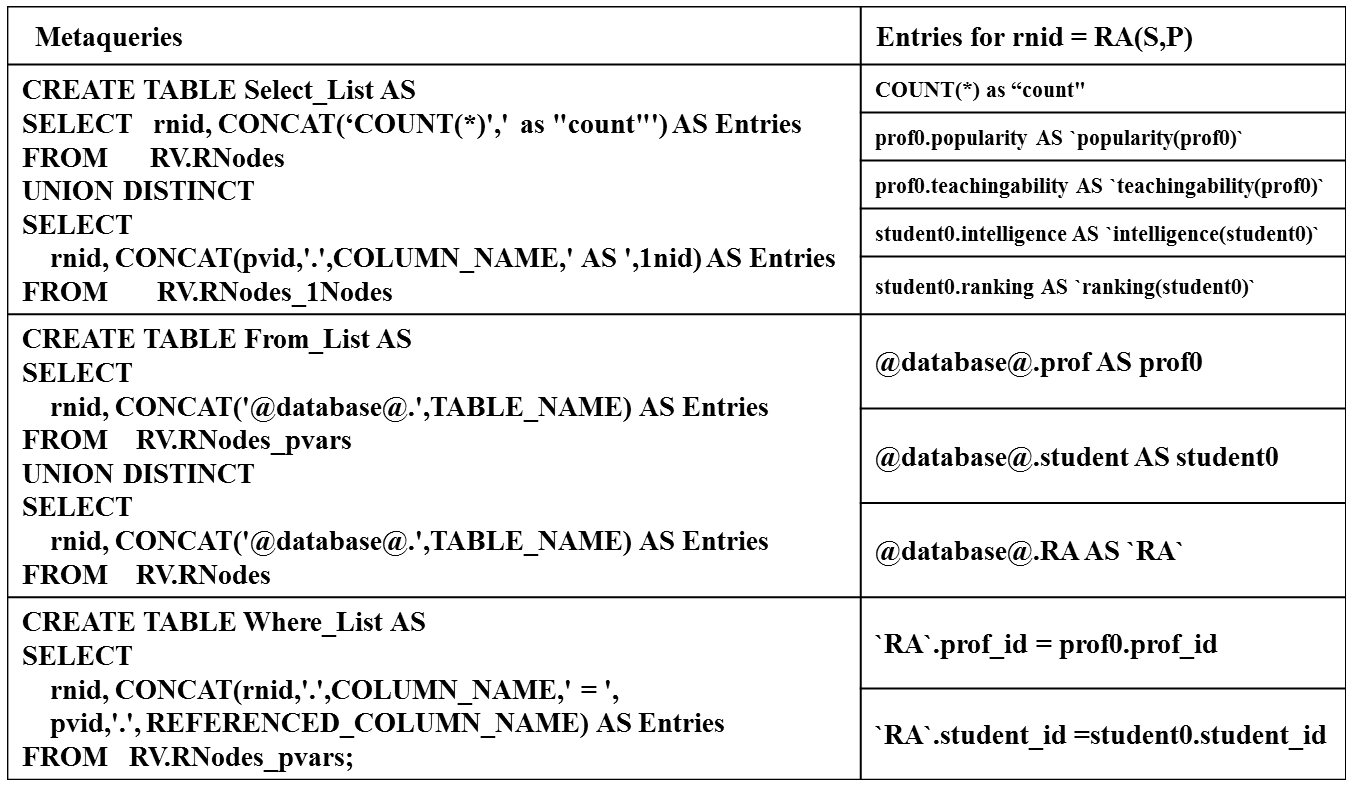
\includegraphics[width=0.5\textwidth]{figures/meta-query.png}
}
\caption{Example of metaqueries and metaquery results for the relationship table $\ra$  based on university database.
~\label{fig:meta-query} }
\end{center}
\end{figure}


\section{Computing Contingency Tables For Negative Relationships} \label{sec:cta}

Computing sufficient statistics that involve negative relationships is infeasible using standard table joins. 
%and can be carried out by regular table joins or optimized virtual joins~\cite{Yin2004}. 
%
%Computing joint probabilities for a family containing one or more negative relationships is harder. 
Standard join tables materialize new data tables that enumerate tuples of objects that are {\em not} related. %(see Figure~\ref{fig:university-tables}).
%and then apply existing counting methods to the new tables. 
However, the number of unrelated tuples is too large to make this scalable (consider the number of user pairs who are {\em not} friends on Facebook). 
%A numerical example will illustrate why this is not feasible. Consider a university database with 20,000 Students, 1,000 Courses and 2,000 TAs. If each student is registered in 10 courses, the size of a $\it{Registered}$ table is 200,000. So the number of complementary student-course pairs is $2 \times 10^{7}-2 \times 10^{5}$, which is too big for most database systems. 
%If we consider joins, complemented tables are even more difficult to deal with: suppose that each course has at most 3 TAs. Then  the number of satisfying instantiations of a positive relationship only formula such as $\it{Registered}(\S,\C) = \true,\it{TA}(\T,\C) = \true)$ is less than $6 \times 10^{5}$, whereas with negations the number of instantiations of the expression $\it{Registered}(\S,\it{course}) = \false, \it{TA}(\T,\it{course}) = \false)$ is on the order of $4 \times 10^{10}$. 
%\subsection{The M\"obius parametrization.} 
%To compute frequencies involving negative relationships, we would like to use the optimized algorithms for table join frequencies as an oracle/black box. 
%Can we instead reduce the computation of sufficient statistics that involve negative relationships to the computation of sufficient statistics that involve existing (positive) relationships only? 
%In their work on learning Probabilistic Relational Models with existence  uncertainty, Getoor et al. 
%provided a subtraction method for the special case of estimating counts with only a single negative relationship \cite[Sec.5.8.4.2]{Getoor2007c}. 
%They did not treat contingency tables with multiple negative relationships, which we consider next.

We describe a virtual join algorithm that computes the required data tables without the quadratic cost of materializing a cross-product. Our experiments below compare the virtual joins with materializing table joins. 
%We approach this problem in two steps. 
First, we introduce a new extension of relational algebra that we term \textbf{contingency table algebra}. The purpose of this extension is to 
show that query counts using $m+1$ negative relationships can be computed from two query counts that each involve at most $m$ relationships. 
%We state this result as a relational algebra identity in a new extension of relational algebra that we term \textbf{contingency table algebra}. 
Second, a dynamic programming algorithm applies the algebraic identify repeatedly to efficiently build up a complete contingency table from partial tables.
% that involve fewer negative relationships. 

%Our first naive implementation constructs this tables using standard joins. 
%While this was sufficient for our experiments, the cross-products carry a \textbf{quadratic} costs for binary relations, and therefore do not scale to large datasets. 
%Moreover, the hierarchical search requires joins of the extended tables. 



%
%Our starting point is the observation that a statistical learning algorithm like a Bayes net learner does not require an enumeration of individuals tuples, but only {\em sufficient statistics} \cite{Heckerman1995,Schulte2011}. 
%These can be represented in {\em contingency tables} as follows \cite{Moore1998}. 
%Consider a fixed list of relationship nodes $\R_{1}, R_{2},\ldots,R_{m}$, and attribute nodes $\functor_{1},\ldots,\functor_{j}$. 
%A \textbf{query} is a set of $(node = value)$ pairs where each value is of a valid type for the node. 
%The \textbf{result set} of a query in a database $\D$ is the set of instantiations of the first-order variables such that the query evaluates as true in $\D$.
%For example, in the database of Figure~\ref{fig:university-tables} the result set for the query 
%$(\it{intelligence}(\S) = 2$, $\it{rank}(\S) = 1$, $\it{rating}(\C) = 3$, $\it{Diff}(C) = 1$, $\reg(\S,\C) = F)$ 
%is the singleton $\{\langle \it{kim}, \it{101}\rangle\}$. 
%The \textbf{count} of a query is the cardinality of its result set. 
%Each subset of nodes $\set{V} = v_{1},\ldots,v_{n}$ has an associated \textbf{contingency table} denotes by $\cttable(\set{V})$. %$CT(\set{V})$. 
%This is a table with a row for each of the possible assignments of values to the nodes in $\set{V}$, and a special integer column called $\qcount$. 
%The value of the $\qcount$ column in a row corresponding to $V_{1} = v_{1},\ldots,V_{n} = v_{n}$ records the count of the corresponding query. 
%Figure~\ref{fig:ct} shows a partial contingency table from University database.





\subsection{Contingency Table Algebra} \label{sec:cta}

We introduce relational algebra style operations defined on contingency tables.
%\subsection{Definition} 
%First we introduce some notation.
%If $\dtable$ denotes a generic database table, then $\ColumnList(\dtable)$ is a list of columns in table $\dtable$; the list order is irrelevant. For a CT-table $\ct$, the expression $\ColumnList(\ct)$ denotes a list of columns other than the count column.

%none $\qcount$ columns in table $\dtable$, 
%and column sets $\set{V}$, $\set{U}$ are the union of $ \qcount $ column with $\ColumnList({\dtable})$ for different given $\dtable$. 
%Suppose ${\dtable}_{1}$, ${\dtable}_{2}$ be two union-compatible %contingency 
%tables with the same column headers, and ${\dtable}_{3}$ is another table,
%then $\ColumnList({\dtable}_{1}) =V_{1}, \ldots,\ V_{k}$, $\ColumnList({\dtable}_{2}) =V_{1}, \ldots,\ V_{k}$
%and $\ColumnList({\dtable}_{3}) = U_{1}, \ldots,\ U_{m}$.
%We define $\ColumnList({\dtable}_{1}) = \ColumnList({\dtable}_{2})$ by 
%${\dtable}_{1}.V_{1} ={\dtable}_{2}.V_{1}, \ldots, {\dtable}_{1}.V_{k} = {\dtable}_{2}.V_{k}$.


\subsubsection{Unary Operators} \label{sec:unary}
\begin{description}
\item[Selection] $\sigma_{\selectcond}  \ct$ selects a subset of the rows in the  $\ct$-table  that satisfy condition $\selectcond$. This is the standard relational algebra operation except that the selection condition $\selectcond$ may not involve the $\qcount$ column.
\item[Projection]  %$\project_{\set{V}}  
$\project_{\V_{1},\ldots,\V_{k}} \ct$ selects a subset of the  columns in the  $\ct$-table, excluding the count column. 
The counts in the projected subtable are the sum of counts of rows that satisfy the query in the subtable. 
The  $\ct$-table projection  $\project_{\V_{1},\ldots,\V_{k}} \ct$ can be defined by the following pseudo-SQL code:

\begin{quote}
SELECT SUM(COUNT) AS COUNT, $V_{1}, \ldots,\ V_{k}$ \\
FROM $\ct$ \\
GROUP BY $V_{1}, \ldots,\ V_{k}$
\end{quote}
%\begin{quote}
%SELECT SUM($\qcount$) AS $\qcount$, $\ColumnList({\ct})$ \\
%FROM $\ct$ \\
%GROUP BY $\ColumnList({\ct})$
%\end{quote}


\item[Conditioning]  $\condition_{\selectcond}  \ct$ returns a conditional contingency table. Ordering the columns as $(V_{1},\ldots,V_{k}, \ldots,\V_{k+j}$),  suppose that the selection condition is a conjunction of values of the form $C = (V_{k+1} = v_{k+1},\ldots, V_{k+j} = v_{k+j})$.  Conditioning can be defined in terms of selection and projection by the equation:
\begin{equation}
\condition_{\selectcond}  \ct = \project_{\V_{1},\ldots,\V_{k}} (\select_{\selectcond}  \ct) \nonumber
\end{equation}
\end{description}

\subsubsection{Binary Operators} \label{sec:bin}
With some abuse of notation, we use $\set{V}$ in pseudo-SQL to denote a list of column names in arbitrary order. The notation $\ct_{1}.\set{V} = \ct_{2}.\set{V}$ indicates an equijoin condition: the contigency tables $\ct_{1}$ and $\ct_{2}$ have the same column set $\set{V}$ and matching columns from the different tables have the same values.
\begin{description}
\item[Cross Product]  %Let %$\ct_{1}(\V_{1}, \ldots,\ V_{m}),\ct_{3}(U_{1}, \ldots,\ U_{k})$
%$\ct_{1}(\set{V}),\ct_{3}(\set{U})$ 
% be two contingency tables %that do not share any papulation variable. 
The \textbf{cross-product} of $\ct_{1}(\set{U}),\ct_{2}(\set{V})$ is the Cartesian product of the rows, where the product counts are the products of count. The cross-product can be defined by the following pseudo-SQL code:
% \begin{quote}
%SELECT \\($\ct_{1}.COUNT*\ct_{2}.COUNT$) AS COUNT,  $U_{1}, \ldots,\ U_{k}, \V_{1}, \ldots,\ V_{m}$ \\
%FROM  $\ct_{1},\ct_{2}$
%\end{quote}
\begin{quote}
SELECT \\($\ct_{1}.\qcount *\ct_{2}.\qcount$) AS $\qcount$,  $\set{U}$, $\set{V}$\\
FROM  $\ct_{1},\ct_{2}$
\end{quote}


\item[Addition] 
 The \textbf{count addition} $\ct_{1}(\set{V}) + \ct_{2}(\set{V})$ adds the counts of matching rows, as in the following pseudo-SQL query.
\begin{quote}
SELECT % $\ct_{1}$.COUNT+$\ct_{2}$.COUNT 
$\ct_{1}.\qcount$+$\ct_{2}.\qcount$ AS $\qcount$, $\set{V}$ \\%$\ct_{1}.V_{1} , \ldots, \ct_{1}.V_{k} $ \\
FROM  $\ct_{1},\ct_{2}$\\
%WHERE $\ct_{1}.V_{1} = \ct_{2}.V_{1}, \ldots, \ct_{1}.V_{k} = \ct_{2}.V_{k}$
WHERE $\ct_{1}.\set{V} = \ct_{2}.\set{V}$
\end{quote}

If a row appears in one $\ct$-table but not the other, we include the row with the count of the table that contains the row. %Note that  $\ct_{1}(\set{V})$ and $\ct_{2}(\set{V})$ are union-compatible because they have the same  column headers.

\item[Subtraction] %Let $\ct_{1}(\set{V}),\ct_{2}(\set{V})$ be two union-compatible contingency tables with the same column headers. 
The \textbf{count difference} $\ct_{1}(\set{V}) - \ct_{2}(\set{V})$ equals $\ct_{1}(\set{V}) + (- \ct_{2}(\set{V}))$ where $- \ct_{2}(\set{V})$ is the same as $\ct_{2}(\set{V})$ where the counts are negative. 
Table subtraction is defined only if (i) without the $\qcount$ column, the rows in $\ct_{1}$ are a superset of those in $\ct_{2}$, and (ii) for each row that appears in both tables, the count in $\ct_{1}$ is at least as great as the count in $\ct_{2}$.


\end{description}


%\subsection{Implementing the Contingency Table Operators}\label{sec:imp}
%Everything true: database optimization. General tricks, e.g., omit 0 counts. Specific tricks, e.g. merge-sort.
\subsubsection{Implementation}\label{sec:imp}
Our implementation is based on SQL queries, whose execution is well optimized by a RDBMS such as MySQL.   
%A RDBMS offers built-in options for improving query planning, such as using covering index  to speed up the conditioning.
%[give examples: e.g, indixes]. 
For some operations where MySQL chooses a suboptimal query plan, we implemented our own method.

%\subsubsection{Unary Operators}
%Suppose we already know the required columns list $\ColumnList({\dtable})$ for each query clause. 
The selection operator can be implemented  using SQL as with standard relational algebra. 
Project with $\ct$-tables requires use of the GROUP BY construct as shown in Section~\ref{sec:unary}. 
%The list of columns to be projected at a point in the algorithm can be found by a meta query. 
%\subsubsection{Binary Operators}
 % big * smaller, faster enough.
%The required column lists can be found by a meta query. 

%The most difficult operation to implement efficiently is 
For addition/subtraction, simply executing the SQL query shown above %shown in Section~\ref{sec:bin} 
may lead to a \textbf{quadratic} cost if a nested-loops join is used, and therefore does not scale to large datasets.
A more efficient algorithm is a sort-merge join \cite{Ullman1982}. 
Given two union-compatible $\ct$-tables, each row in one matches at most one other on the non-count columns. 
As is well known, with unique matches, the cost of a sort-merge join is $\it{size}(table1) + \it{size}(table2) +$ the cost of sorting both tables. 
Our experiments below are based on a sort-merge join (our own implementation in Java). 

The cross product is easily implemented in SQL as shown in Section~\ref{sec:bin}. The cross product size is quadratic in the size of the input tables, so a quadratic cost is unavoidable.
%A general trick to shrink the size $\ct$-table is remove the 0 counts in $\ct$-table.
%But for a general input database, usually the user can not know the column lists in advance. 
%So in next section, we propose a new method to compute these.





\subsection{Latttice Computation of Contingency Tables} \label{sec:mobius}


%\textbf{older material}
%Our flat search algorithm can be implemented by computing the contingency table for all functor nodes, then presenting it to a Bayes net learner. 
%The hierarchical search algorithms can be implemented by computing the contingency tables for each relationship chain in the lattice (Figure~\ref{fig:big-lattice}). 
%For a relationship set, the nodes in the contingency table comprise (1) the descriptive attributes of the entities involved in the relationship set, 
%(2) the descriptive attributes of the relationships, and (3) a Boolean relationship node for each member of the set. 
This section describes a method for computing the contingency tables level-wise in the relationship chain lattice. We start with a contingency table algebra equivalence that allows us to compute counts for rows with negative relationships from rows with positive relations.
%
%
%\textbf{old material} So long as a database probability involves only positive relationships,
%%formula only contains positive relationships, 
%%the computation is straightforward. 
%%For example, in 
%%$P_{\D}(\it{gender}(\X) = M, \it{Friend}(\X,\Y) = \true)$, the value  $\grounds_{\D}(\it{gender}(\X) = M, \it{Friend}(\X,\Y) = \true)$, the count of friendship pairs $(x,y)$ where $x$ is male and the
%%{\em Friend} relationship is true, 
%and can be carried out by regular table joins or optimized virtual joins~\cite{Yin2004}. 
%%
%Computing joint probabilities for a family containing one or more negative relationships is harder. 
%A naive approach would explicitly construct new data tables that enumerate tuples of objects that are {\em not} related. %(see Figure~\ref{fig:university-tables}).
%%and then apply existing counting methods to the new tables. 
%However, the number of unrelated tuples is too large to make this scalable (think about the number of user pairs who are {\em not} friends on Facebook). 
%A numerical example will illustrate why this is not feasible. Consider a university database with 20,000 Students, 1,000 Courses and 2,000 TAs. If each student is registered in 10 courses, the size of a $\it{Registered}$ table is 200,000. So the number of complementary student-course pairs is $2 \times 10^{7}-2 \times 10^{5}$, which is too big for most database systems. 
%If we consider joins, complemented tables are even more difficult to deal with: suppose that each course has at most 3 TAs. Then  the number of satisfying instantiations of a positive relationship only formula such as $\it{Registered}(\S,\C) = \true,\it{TA}(\T,\C) = \true)$ is less than $6 \times 10^{5}$, whereas with negations the number of instantiations of the expression $\it{Registered}(\S,\it{course}) = \false, \it{TA}(\T,\it{course}) = \false)$ is on the order of $4 \times 10^{10}$. 
%\subsection{The M\"obius parametrization.} 
%To compute frequencies involving negative relationships, we would like to use the optimized algorithms for table join frequencies as an oracle/black box. 
%Can we instead reduce the computation of sufficient statistics that involve negative relationships to the computation of sufficient statistics that involve existing (positive) relationships only? 
%In their work on learning Probabilistic Relational Models with existence  uncertainty, Getoor et al. 
%provided a subtraction method for the special case of estimating counts with only a single negative relationship \cite[Sec.5.8.4.2]{Getoor2007c}. 
%They did not treat contingency tables with multiple negative relationships, which we consider next.
%
Following \cite{Moore1998}, we use a ``don't care" value $*$ to indicate that a query does not specify the value of a node. For instance, the query $\Relation_{1} = \true, \Relation_{2} = *$ is equivalent to the query $\Relation_{1} = \true$.

\begin{proposition}%[Pivot_CT]
\label{PivotCT}
Let $R$ be a relationship node and let $\set{R}$ be a set of relationship nodes. Let $\Nodes$ be a set of nodes that %(1) must contain all $\eatts$ of $\R$, and may contain any other nodes, as long as (2) $\Nodes$ 
does not contain $\R$ nor any of the $\ratts$ of $\R$. Let  $\X_{1},\ldots, \X_{l}$ be the first-order variables that appear in $\R$ but not in $\Nodes$, where ${l}$ is possibly zero. Then we have
\begin{flalign}
\label{update}
&\ct(\Nodes \cup \eatts(R)|\set{R} = \true, R = F) = & \\ %\nonumber\\
& \ct(\Nodes|\set{R} = \true, R =*) \times \ct(\X_{1}) \times \cdots \times \ct(\X_{l}) \nonumber & \\
& -\ct(\Nodes  \cup \eatts(R)|\set{R} = \true, R = T). \nonumber&
\end{flalign}
If $l = 0$, the equation holds without  the %$ \ct(\X_{1}) \times \cdots \times \ct(\X_{k})$ 
cross-product term.

\end{proposition}
Figure~\ref{fig:flow} illustrates using this equation to build the $\ct_{\false}$ table.

\begin{proof}
The equation 
\begin{align}
&\ct(\Nodes  \cup \eatts(R)|\set{R} = \true, R = *) = &\label{eq:update}  \\ 
&\ct(\Nodes  \cup \eatts(R)|\set{R} = \true, R = T)  + & \nonumber \\ 
&\ct(\Nodes  \cup \eatts(R)|\set{R} = \true, R = F) & \nonumber
\end{align}
holds because the set $\Nodes \cup \eatts(R)$ contains all first-order variables in $R$ by the assumption that each first-order variable is associated with at least one $\eatt .$ % $\it{1Node}$. 

%Using table subtraction Equation~\eqref{eq:update} implies
 Equation~\eqref{eq:update} implies
\begin{align} 
&\ct(\Nodes  \cup \eatts(R)|\set{R} = \true, R = \false) =& \label{eq:table-subtract} \\ 
&\ct(\Nodes  \cup \eatts(R)|\set{R} = \true, R = *) -&\nonumber  \\
 & \ct(\Nodes  \cup \eatts(R)|\set{R} = \true, R = \true).& \nonumber
\end{align}

To compute the $\ct$-table conditional on the relationship $\R$ being unspecified, we use the equation
\begin{align}
&\ct(\Nodes  \cup \eatts(R)|\set{R} = \true, R = *) =  &\label{eq:table-multiply}\\
&\ct(\Nodes|\set{R} = \true, R =*) \times \ct(\X_{1}) \times \cdots \times \ct(\X_{l})& \nonumber
\end{align}
which holds because if the set $\Nodes$ does not contain a first-order variable of $\R$, then the counts of the associated $\eatts(\R)$ are independent of the counts for $\Nodes$. 
If $l = 0$, this means there's no new papulation variable introduced, Equations~\eqref{eq:table-multiply} holds without  the cross-product term.

Together Equations~\eqref{eq:table-subtract} and~\eqref{eq:table-multiply} establish the proposition \ref{PivotCT}.
\end{proof}


\begin{algorithm}[htbp]
\label{Pivot_CT_Computation}
%\linesnumbered
\SetKwData{KwCalls}{Calls}
\SetKwData{KwCondition}{Precondition:}
\KwIn{Two conditional contingency tables   $\ct_{\true} :=\ct(\it{Nodes},\it{\ratts}(R_{\it{pivot}})|R_{\it{pivot}}=\true$$,\vec{R}=\true)$ and  $\ct_{*} :=\ct(\it{Nodes}|R_{\it{pivot}} = *$$,\vec{R}=\true)$ .}
\KwCondition  %$\it{Nodes}:= \eatts(\R_{1},\ldots,\R_{\ell}) \cup \ratts(\R_{1},\ldots,\R_{\ell}) \cup (\R_1,\ldots,\R_{\ell}) - R_{\it{pivot}} - \ratts(R_{\it{pivot}}) $ \;
 The set $\it{Nodes}$ does not contain the relationship node $R_{\it{pivot}}$ nor any of its descriptive attributes $\ratts(R_{\it{pivot}}$).

% {The set $\it{Nodes}$ contains $\eatts(\R_{1},\ldots,\R_{\ell}) \cup \ratts(\R_{1},\ldots,\R_{\ell}) \cup (\R_1,\ldots,\R_{\ell})$ but not the relationship node $R_{\it{pivot}}$ nor any of its descriptive attributes $\ratts(R_{\it{pivot}}$) \;}

\KwOut{The conditional contigency table $ \ct(\it{Nodes},\it{\ratts}(R_{\it{pivot}}),R_{\it{pivot}}|$$\vec{R}=\true)$ .}
\begin{algorithmic}[1]
%\STATE $CT_{\false} := \ct(\it{Nodes}|R_{\it{pivot}} = *$$,\vec{R}=\true) - \pi_{\it{Nodes}} \ct(\it{Nodes},\it{\ratts}(R_{\it{pivot}})|R_{\it{pivot}}=\true$$,\vec{R}=\true)$.
\STATE $\ct_{\false} := \ct_{*} - \pi_{\it{Nodes}}\ct_{\true}$.

\COMMENT{Implements the algebra Equation~\ref{update} in proposition~\ref{PivotCT}.}
\STATE $\ct_{\false}^{+}$ := extend  $\ct_{\false}$ with columns $R_{\it{pivot}}$ everywhere false and $\it{\ratts}(R_{\it{pivot}})$ everywhere $n/a$.
%\STATE $CT_{\true}^{+}$ := extend  $\ct(\it{Nodes},\it{\ratts}(R_{\it{pivot}})|R_{\it{pivot}}=\true$$,\vec{R}=\true)$ with columns $R_{\it{pivot}}$ everywhere true.
\STATE $\ct_{\true}^{+}$ := extend  $\ct_{\true}$ with columns $R_{\it{pivot}}$ everywhere true.
\STATE \Return $\ct_{\false}^{+} \cup \ct_{\true}^{+}$
\end{algorithmic}
\label{alg:pivot}
\caption{The Pivot function returns a conditional contingency table for a set of attribute nodes and all possible values of the relationship $R_{\it{pivot}}$, including $R_{\it{pivot}} = \false$. %It implements the algebra Equation~\eqref{eq:update}.
 The set of conditional relationships $\vec{R} =(\R_{pivot},\ldots,\R_{\ell})$ %=\true$
 may be empty in  which case the Pivot computes an unconditional ct-table. }
\end{algorithm}





Algorithm~\ref{Pivot_CT_Computation} provides pseudo-code for applying Equation~\eqref{eq:update} to compute a complete $\ct$-table given a partial table where a specified relationship node $\Relation$  is true
and another partial table that does not contain the relationship node. 
We refer to $\Relation$ as the \textbf{pivot} node. 
For extra generality, we apply the Equation with a condition that lists a set of relationship nodes fixed to be true.  
Algorithm~\ref{level-wise-subtract} shows how the Pivot operation can be applied repeatedly to find all contigency tables in the relationship lattice. Figure~\ref{fig:flow} illustrates the computation for the case of only one relationship. The computation for any number of relationships proceeds as follows. 



\begin{algorithm}[!h]
\label{level-wise-subtract}
\SetKwData{KwCalls}{Calls}
\SetKwData{Notation}{Notation}
\KwIn{A relational database $\D$; a set of functor nodes}
\KwOut{A contingency table that lists the count in the database $D$ for each possible assignment of values to each functor node.}
\begin{algorithmic}[1]
\FORALL{first-order variables $\X$}
\STATE compute $\ct(\eatts(\X))$ using SQL queries.
\ENDFOR
\FORALL{relation node $\R$}
\STATE $\ct_{*} := \ct(\X) \times \ct(\Y)$ where $\X$,$\Y$ are the first-order variables in $\R$.
\STATE $\ct_{\true} := \ct(\eatts(\R)|\R = \true)$ using SQL joins.
\STATE Call  $\it{Pivot}(\ct_{\true},\ct_{*})$ to compute $\ct(\eatts(\R),\ratts(\R),\R)$.
\ENDFOR
\FOR{Rchain length $\ell=2$ to $m$}
\FORALL{Rchain $\R_{1},\ldots,\R_{\ell}$}
\STATE $Current\_\ct :=  \ct(\eatts(\R_{1},\ldots,\R_{\ell}),$
	\\$\ratts(\R_{1},\ldots,\R_{\ell})|\R_{1}=\true,\ldots,\R_{\ell}=\true)$ \\
\COMMENT{using SQL joins.}
\FOR{$i=1$ to $\ell$} \label {refline:innerloop}
\IF{ $i$ equals  1}
\STATE $\ct_{*} := \ct(\eatts(\R_{2},\ldots,\R_{\ell}),\ratts(\R_{2},\ldots,\R_{\ell})$ \\$|
\R_{1}=*,\R_{2} = \true,\ldots,\R_{\ell}=\true) \times \ct(\X)$ where $\X$ is the first-order variable in $\R_{1}$, if any, that does not appear in $\R_{2},\ldots,\R_{\ell}$\; 
\COMMENT{$\ct_{*}$ can be computed from a $\ct$-table for a Rchain of length $\ell-1$.}
\ELSE
\STATE $\eatts_{\bar{i}} := \eatts(\R_{1},\ldots,\R_{i-1},\R_{i+1},\ldots,\R_{\ell})$.
\STATE $\ratts_{\bar{i}} := \ratts(\R_{1},\ldots,\R_{i-1},\R_{i+1},\ldots,\R_{\ell})$.
\STATE $\ct_{*} := \ct(\eatts_{\bar{i}}, \ratts_{\bar{i}},\R_{1},\ldots,\R_{i-1})$\\$|
\R_{i}=*,\R_{i+1} = \true,\ldots,\R_{\ell}=\true) \times \ct(\Y)$ where $\Y$ is the first-order variable in $\R_{i}$, if any, that does not appear in $\vec{\R}$. 
\ENDIF \\
\STATE $Current\_\ct :=  \it{Pivot}(Current\_\ct,\ct_{*})$.
\ENDFOR \;
\COMMENT{Loop Invariant: After  iteration $i$, the table $Current\_\ct$ equals 
$\ct(\eatts(\R_{1},\ldots,\R_{\ell}), \ratts(\R_{1},\ldots,\R_{\ell}),$\\$\R_{1},\ldots,\R_{i}|\R_{i+1} = \true,\ldots,\R_{\ell}=\true)$}
\ENDFOR
\COMMENT{Loop Invariant: The $\ct$-tables for all Rchains of length $\ell$ have been computed.}
\ENDFOR 
\STATE \Return the $\ct$-table for the Rchain involves all the relationship nodes.
\end{algorithmic}
\label{alg:fmt}
\caption{Virtual Join Algorithm for Computing the Contingency Table for Input Database}%Dynamic Algorithm for Computing  {\em Sufficient Statistics} given one relational database }
\end{algorithm}

{\em Initialization.} Compute $\ct$-tables for entity tables.
% (lines 1--3). 
Compute $\ct$-tables for each single relationship node $\Relation$ , conditional on $\Relation = \true$. % (line 6).  
If $\Relation = \ast$, then no link is specified between the first-order variables involved in the relation $\Relation$. Therefore the individual counts for each first-order variable are independent of each other and the joint counts can be obtained by the cross product operation. % (line 5). 
Apply the Pivot function to construct the  complete $\ct$-table for each relationship node $\Relation$. % (line 7). 

{\em Lattice Computation.} The goal is to compute $\ct$-tables for all relationship chains of length $>1$. For each relationship chain, order the relationship nodes in the chain arbitrarily. Make each relationship node in order the Pivot node $\Relation_{i}$. For the current Pivot node $\Relation_{i}$, find the conditional $\ct$-table where $\Relation_{i}$ is unspecified, and the subsequent relations $\Relation_{j}$ with $j>i$ are true. This $\ct$-table can be computed from a $ct$-table for a shorter chain that has been constructed already. Now the conditional $ct$-table  where $\Relation_{i}$ is true, and the subsequent relations are true, has been constructed already (see loop invariant). Apply the Pivot function to construct the  complete $\ct$-table, for any value of the Pivot node $\Relation_{i}$,  conditional on the subsequent relations being true.




\begin{figure*}[tb]
\begin{center}
\resizebox{0.9\textwidth}{!}{
%%!%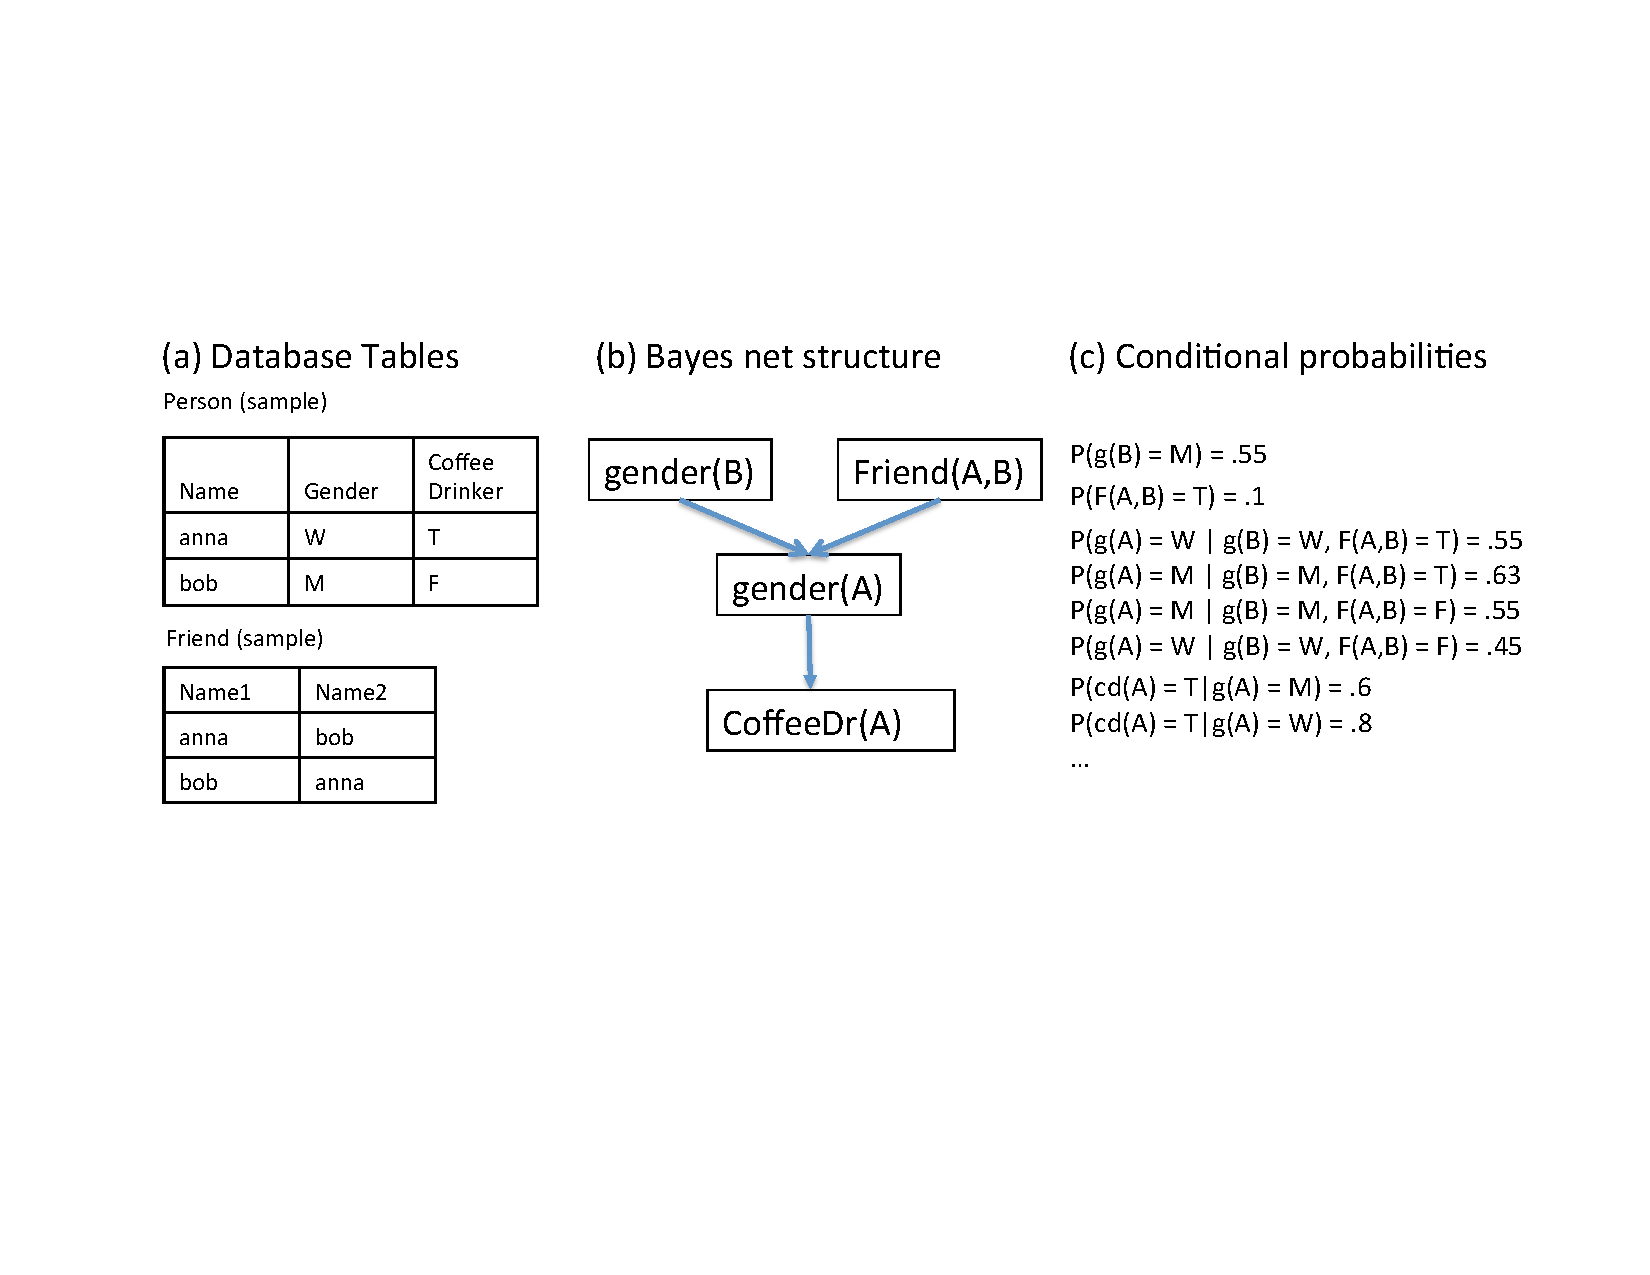
\includegraphics[width=1\textwidth]{pbn}
%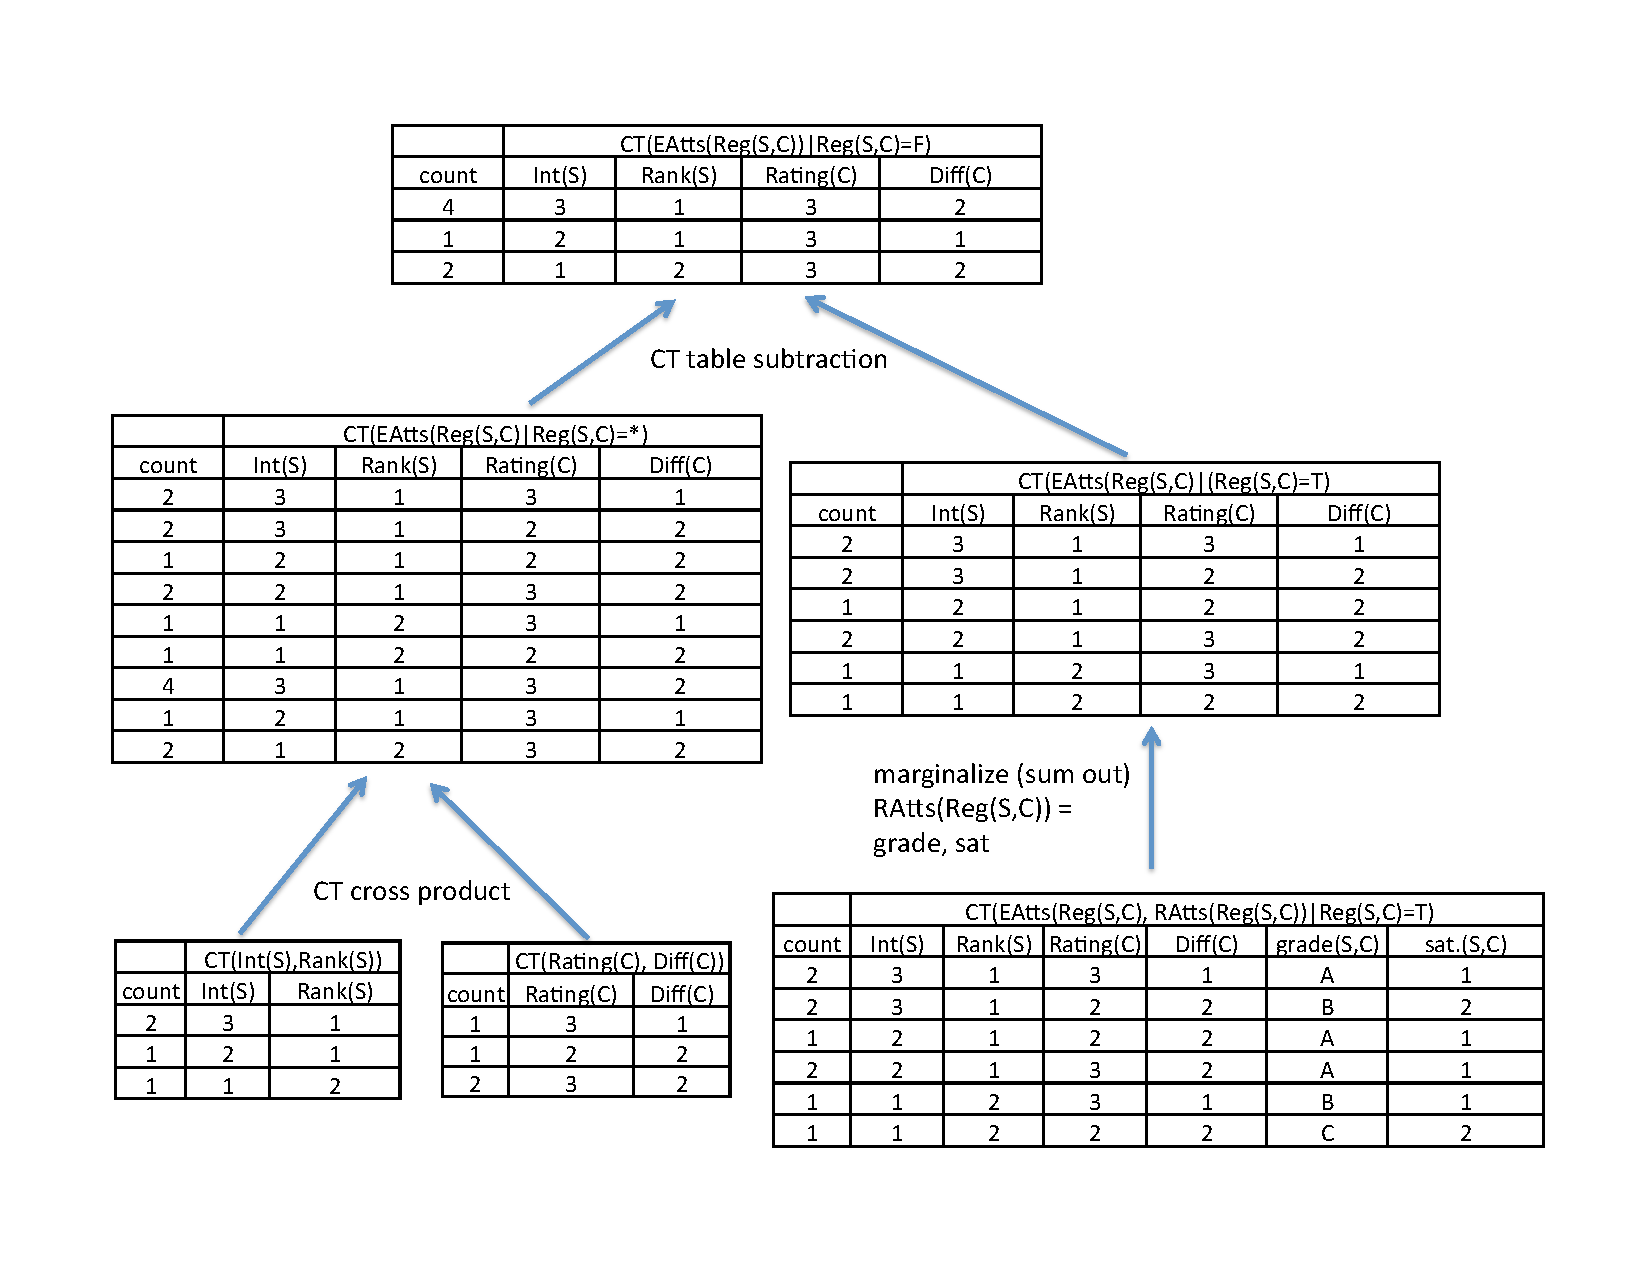
\includegraphics{figures/subtraction-flow.pdf}
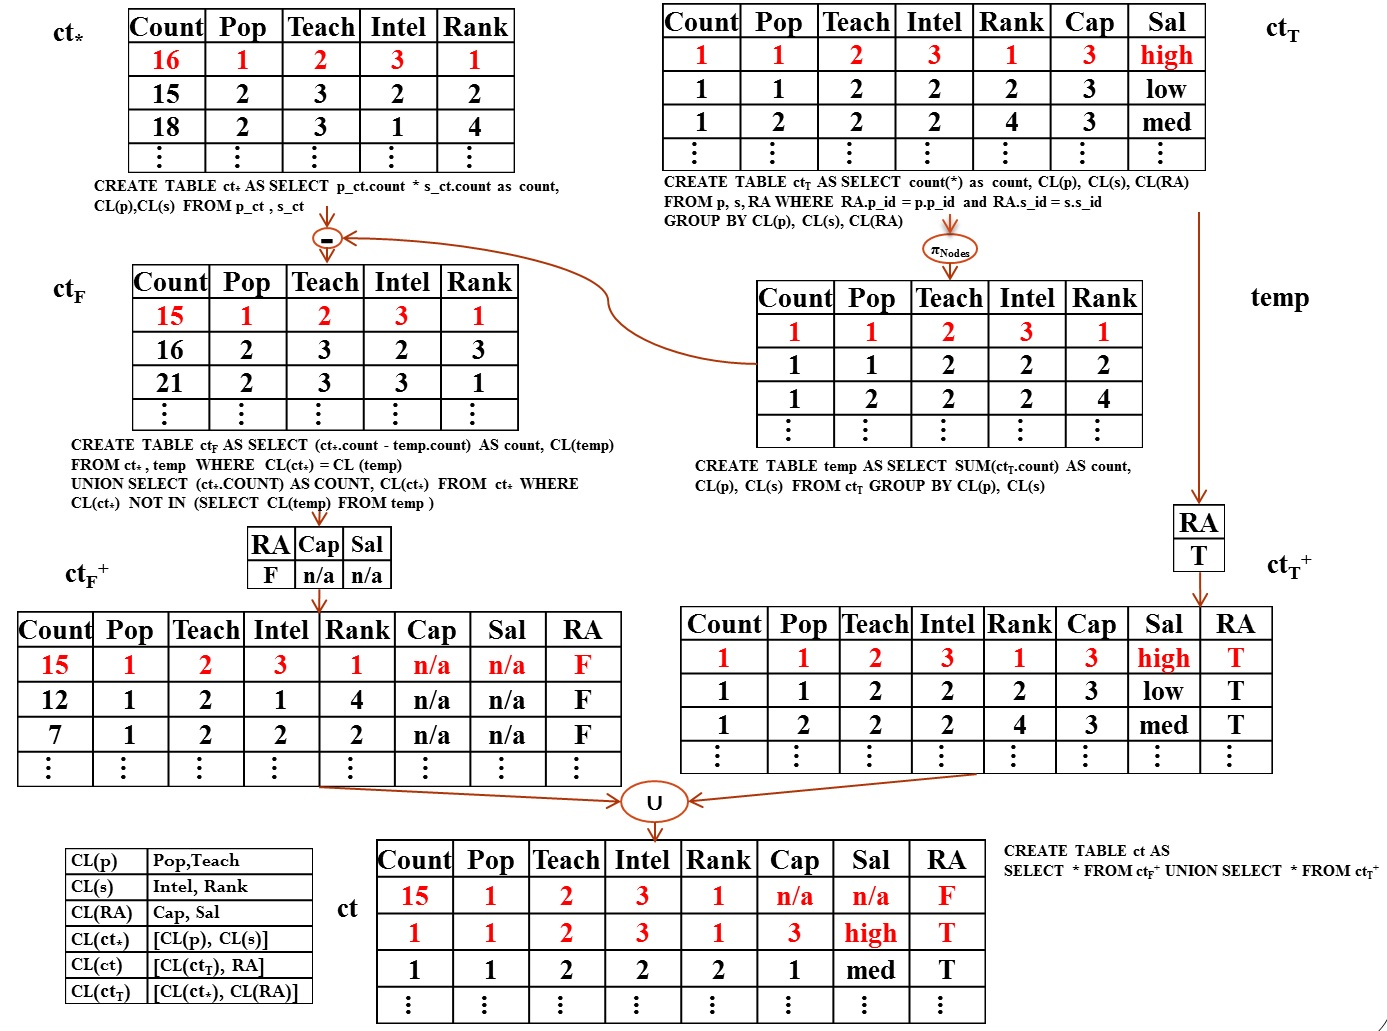
\includegraphics[width=0.9\textwidth]{figures/sub.jpg}
}
\caption{Computation of the $\ct$-table for the Rnode $\ra(\S,\P)$ using Algorithm~\ref{Pivot_CT_Computation}. The operations are implemented using dynamic SQL queries as shown. Lists of column names are abbreviated as shown and as follows.
$\ColumnList({\ct_{*}}) = \ColumnList({temp})=\ColumnList({\ct_{F}})$, 
$\ColumnList({\ct}) =  \ColumnList(\ct_{\false}^{+})  = \ColumnList(\ct_{\true}^{+}) $.
\label{fig:flow}}
\end{center}
\end{figure*}








\subsubsection{Complexity Analysis} 

The key point about the Virtual Join Algorithm %(VJA) %~\ref{alg:fmt} 
is that it avoids the generally infeasible enumeration of tuples of entities that are not related.
{\em The algorithm accesses  only \textbf{existing} tuples, never constructs nonexisting tuples.}

To  analyze the computational cost, we examine the total number of $\ct$-algebra operations performed by the Virtual Join Algorithm. 
%In the next section we discuss the cost of a single  $\ct$-algebra operation.
%
We provide  upper bounds in terms of two parameters: the number of relationship nodes  $m$, and  the number of rows $\row$  in the $\ct$-table that is the output of the algorithm. 
For these parameters we establish that
$$\it{\# \ct\_\it{ops}} = O(r \cdot \log_{2} r) = O(m \cdot 2^{m}) .$$
This shows the efficiency of our algorithm for the following reasons.
(i) Since the time cost of any algorithm must be at least as great as the time for writing the output, which is as least as great as $\row$, 
the Virtual Join Algorithm adds at most a logarithmic factor to this lower bound. 
(ii)  The second upper bound means that the number of $\ct$-algebra operations is fixed-parameter tractable with respect to $m$.\footnote{For arbitrary $m$, the problem of computing a $\ct$ table in a relational structure is \#P-complete \cite[Prop.12.4]{Domingos2007}.} In practice the number $m$ is on the order of the number of tables in the database, 
which is very small compared to the number of tuples in the tables.

\emph{Derivation of Upper Bounds.}
For a given relationship chain of length $\ell$, the Virtual Join Algorithm goes through the chain linearly (Algorithm~\ref{alg:fmt} inner for loop line ~\ref {refline:innerloop}%12
). 
% check line number
At each iteration, it computes a $\ct_{*}$ table with a single cross product, then performs a single Pivot operation.
 Each Pivot operation requires three  $\ct$-algebra operations. 
Thus overall, the number of  $\ct$-algebra operations for a relationship chain of length $\ell$ is $6 \cdot \ell = O(\ell)$. For a fixed length $\ell$, there are at most $\binom{m}{\ell}$ relationship chains. Using the known identity
\begin{align} 
\sum_{\ell=1}^{m} {m\choose \ell} \cdot \ell = m \cdot  2^{m-1} \label{eq:upperbound}
\end{align}
we obtain the $O(m \cdot  2^{m-1}) = O(m \cdot  2^{m})$ upper bound\footnote{http://goo.gl/x65yl3}. 
%\textbf{URL}
%With the Binomial theorem the identity ~\eqref{eq:upperbound} is easy to prove, we omit further details due to space constraints.

For the upper bound in terms of $\ct$-table rows $\row$, we note that the output $\ct$-table can be decomposed into $2^{m}$ subtables, one for each assignment of values to the $m$ relationship nodes. 
Each of these subtables contains the same number of rows $d$ , one for each possible assignment of values to the attribute nodes. 
Thus the total number of rows is given by $r = d \cdot 2^m.$ 
Therefore we have 
$m \cdot 2^{m} = \log_{2} (r/d) \cdot r/d \leq \log_{2}(r) \cdot r.$
Thus the total number of $\ct$-algebra operations is $O(r \cdot \log_{2}(r))$.
%$\it{\# \ct\_\it{ops}} = O(r \cdot \log r) .$

From this analysis we see that both upper bounds are overestimates. (1) Because relationship chains must be linked by foreign key constraints, the number of valid relationship chains of length $\ell$ is usually much smaller than the number of all possible subsets ${m\choose \ell}$. (2) The constant factor $d$ grows exponentially with the number of attribute nodes, so $\log_{2}(r) \cdot r$ is a loose upper bound on $\log_{2} (r/d) \cdot r/d$. 
We conclude that the number of $\ct$-algebra operations is not the critical factor for scalability, but rather the cost of %processing tuples, 
%or in other words, the cost of 
carrying out a single $\ct$-algebra operation. 
In Section~\ref{sec:cta} we discussed how to perform these operations in a scalable manner.
%
%Here we give a quick proof of the identity ~\eqref{eq:upperbound} %or put it in the appendix
%\begin{proof}
%With the Binomial theorem, for any non-negative integers $l,m$, the binomial formula of two variables $a,b$ is 
%$$ f(a,b)=\sum_{\ell=0}^{m}\binom{m}{\ell} \cdot a^{m-\ell} \cdot b^\ell = (a+b)^m. $$
%Suppose we substitute $a$ with one, for any $b$, we have 
%$$
%f(1,b)= \sum_{\ell=0}^m\binom{m}{\ell} \cdot b^\ell=(1+b)^m.
%$$
%And then we could compute the partial derivative with respect to $b$
%$$
%f'_{b}(1,b)= \sum_{\ell=1}^m\binom{m}{\ell}\cdot \ell \cdot b^{\ell-1}=m \cdot (1+b)^{m-1}.$$
%By substituting $b$ with one, we have 
%$$
%f'_{b}(1,1)=  \sum_{\ell=1}^m\binom{m}{\ell}\cdot \ell \cdot 1^{\ell-1}= \sum_{\ell=1}^m\binom{m}{\ell}\cdot \ell = m\cdot(2)^{m-1}.$$
%
%That means the following identity
%$$\sum_{\ell=1}^{m} {m\choose \ell}\cdot \ell = m * 2^{m-1}  $$ holds.
%\end{proof}

\begin{figure}[tbp]
\begin{center}
\resizebox{0.5\textwidth}{!}{
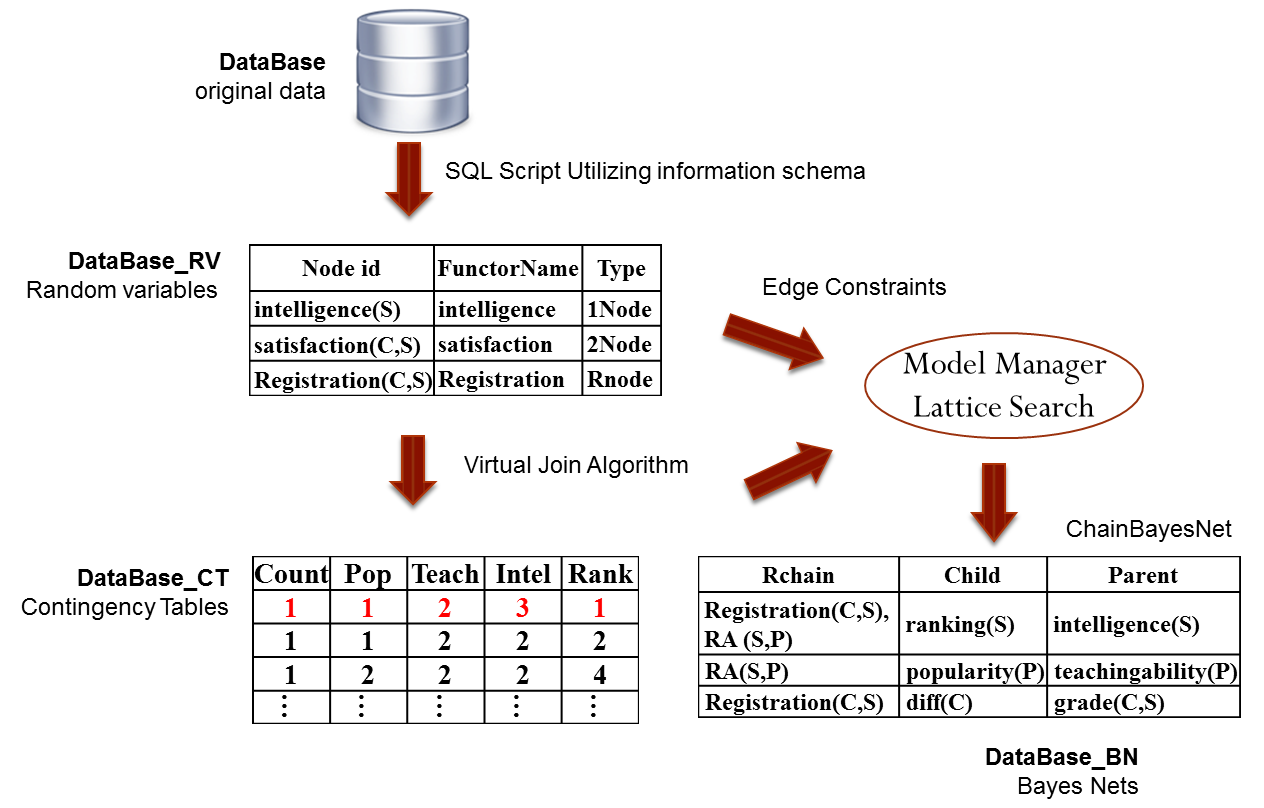
\includegraphics[width=0.8\textwidth]{figures/general-flow-chart.png}
}
\caption{Bayes net structure learning with SQL.
%Here the $DB$ denotes the original database, $DB\_RV$ denotes the database storing all random variables, 
%$DB\_CT$ denotes the database containing all the contingency tables  and $DB\_BN$ storing all the learned Bayes Nets.
\label{fig:general-flow-chart}}
\end{center}
\end{figure}



\section{Application: Bayes Net  Learning }

This section describes an application of our contingency table algorithm to a challenging problem in machine learning: constructing a Bayes net structure for a relational database. Bayes net learning has been considered as an application for caching sufficient statistics for single table data [cite Moore, chinese paper], because computing sufficient statistics is the key factor in scaling Bayes net learning to large datasets [cite Russell and Norvig]. For data exploration, a Bayes net provides a succinct graphical representation of complex statistical-relational correlations. A  Bayes net model supports powerful probabilistic reasoning for answering ``what-if'' queries about the probabilities of uncertain outcomes conditional on observed events. 

%Thus the lattice structure defines a {\em multinet} rather than a single Bayes net. Multinets are a classic Bayes net formalism for modelling {\em context-sensitive} dependencies among variables. They have been applied  for modelling diverse domains, such as sleep disorders, eye diseases, and turbines that generate electricity. 
%Geiger and Heckerman contributed a standard reference article for the multinet formalism  \cite{Geiger1996}.
\subsection{The Learn-and-Join Algorithm} \label{sec:laj}
This Learn-and-Join Algorithm (LAJ)  takes as input a relational database and constructs a Bayes net for each relationship chain. The final Bayes net is the model associated with the largest chain. The LAJ algorithm was previously applied only conditional on all relationship nodes being true. Because our virtual join algorithm provides sufficient statistics about cases where relationship  do not exist, we can extend the LAJ algorithm for learning a Bayes net model of dependencies among relationship nodes. We provide a brief summary; for a detailed description please see \cite{Schulte2011}. The algorithm applies a standard single-table Bayes net learner, which can be chosen by the user, to the contingency table for each chain. 
%Computing the contingency tables is the conceptually and computationally most challenging part of our system. We describe a dynamic programming algorithm for precomputing the contingency tables in Section~\ref{sec:cta} below. In this section we describe the structure learning algorithm on the assumption that the contingency tables have been precomputed.

 The algorithm proceeds level-wise by considering relationship chains of length $\ell = 0,1, 2, \ldots$. After Bayes nets have been learned for length $\ell$, the learned edges are propagated to chains of length $\ell+1$. In the initial case of single relationship tables where $\ell=0$, the edges are propagated from Bayes nets learned for entity tables. Propagated edge constraints are of two types: Required and forbidden edges. 

Suppose that $\rchain$ at level $s$ is a parent of $\rchain'$ at level $s+1$.  For required edges, then if an edge $\node \rightarrow \node'$ is present in the Bayes net $\B_{\rchain}$ for the parent chain $\rchain$, the edge must also contained in the Bayes net $\B_{\rchain'}$ for the child  chain $\rchain'$. In other words, edges present in smaller relationship chains are inherited by larger relationship chains. For forbidden edges, if an edge $\node \rightarrow \node'$ is absent from the Bayes nets of all parent chains of $\rchain'$, it must also be absent from the Bayes net of $\rchain'$. In other words, the absence of edges in smaller relationship chains is inherited by larger relationship chains.

{\em Example.} 
If the $\student$ Bayes net contains an edge $$\it{intelligence}(\S) \rightarrow \it{ranking}(\S),$$ then the Bayes net associated with the relationship $\it{\ra(\S,\C)}$ must also contain this edge (see Figure~\ref{fig:university-tables}). 
If the $\prof$ Bayes net does not contain an edge $$\it{popularity}(\P) \rightarrow \it{teachingability}(\P),$$ it must also be absent in the Bayes net associated with the relationship node $\ra(\P,\S)$.
%If the $\it{Course}$ Bayes net does not contain an edge $$\it{rating}(\C) \rightarrow \it{difficulty}(\C)$$, it must also be absent in the Bayes net associated with the relationship $\it{Registration(\S,\C)}$.




\subsection{Implementation in SQL} 
%\paragraph{The Model Manager: Implementing Hierarchical Model Search in SQL}
%Figure~\ref{figure:flow} illustrates the system flow on part of the relationship lattice. The Bayes net learner receives a CT-table and edge constraints as input, and returns a Bayes net. The view mechanism propagates the results as constraints of learning to larger relationship chains, without the need for any further computation.

The Bayes multinet can be stored in a master table called {\em $ChainBayesNet$}, as shown in Figure \ref{fig:general-flow-chart}. 
An entry such as $$\langle [\reg(\S,\C),\ra(\S,\P)],\it{ranking}(\S),\it{intelligence}(\S)\rangle$$ means that the 
Bayes net graph for the relationship chain $\reg(\S,\C),\ra(\S,\P)$ contains an edge $\it{ranking}(\S)\leftarrow \it{intelligence}(\S)$. 
The Bayes net learner receives a $\ct$-table and edge constraints as input, and returns a Bayes net. The learned edges are exported to the database tables. 
An SQL view defines tables that store the forbidden and required edges: each time that new edges are inserted in the $ChainBayesNet$ table, 
the view mechanism propagates the results as constraints of learning to larger relationship chains, without the need for any further computation. 
The view mechanism provides a compact and flexible update procedure (only 20 lines of SQL code).
Figure~\ref{fig:general-flow-chart} shows the computation flow for our Bayes net learning system. 
After structure learning is complete, the Bayes net parameters can be easily computed from the contingency tables using maximum likelihood estimation, and stored in conditional probability tables in the BN database together with the $ChainBayesNet$ table.


%The SQL View mechanism propagates edges compactly, as shown in Figure~\ref{fig:view-pro}. 
%%The advantage of the view mechanism is that each time that the Bayes net learner completes learning for a lattice point, the view  update mechanism propagates the results as constraints on learning for the children of the lattice point. 
%The {\em LatticeRel} table records which relationship chains are parents of which others. This auxilliary table makes it easy to write a query that finds, for a given child chain, all the parent chains and inserts their edges as entries for the child chain. This view implements the propagation of required edges. The view definition for forbidden edges is similar: the only difference is that we first need to find the set of complement edges that are {\em not} included in the Bayes net of a given relationship chain. The complement edges are also computed by a view (not shown). 



\section{Evaluation} 
All experiments were done on with 8GB of RAM and a single Intel Core 2 QUAD Processor Q6700 with a clock speed of 2.66GHz (there is no hyper-threading on this chip). 
The operating system was Linux Centos 2.6.32. Code was written in Java, JRE 1.7.0. All code and datasets are available~\cite{bib:jbnsite}.
We made use of the following single-table Bayes Net search implementation:  GES search \cite{Chickering2003} with the BDeu score as implemented in version 4.3.9-0 of CMU's Tetrad package (structure prior uniform, ESS=10; \cite{2008a}).
\begin{table}[hbtp] \centering
%\scalebox{0.7in}{
\resizebox{0.5\textwidth}{!}{
\begin{tabular}[c]
{|l|c|c|r|r|}\hline
 \textbf{Dataset} & \textbf{\begin{tabular}[l] {ll} \#Relationship \\Tables \end {tabular}} & \textbf{\begin{tabular}[l] {ll} \#Self \\Relationships\end {tabular}}  & \textbf{\#Tuples} & \textbf{\#Attributes}  \\\hline
% \textbf{Dataset} & \textbf{Relationships} & \textbf{\begin{tabular}[l] {ll} Self \\Relationships \end {tabular}} &
% \textbf{\begin{tabular}[l] {ll} Same Type\\ Relationships \end {tabular}}& \textbf{\#Tuples} & \textbf{\begin{tabular}[l] {ll} \#Attribute  \\Columns \end{tabular}}  \\\hline
 %   University&2 & 0 & N & 171 & 12\\\hline
    Movielens &1 & 0  & 1,010,051 & 7\\\hline
%    Movielens(0.1M) &1 & N & N &  83,402 & 7\\\hline
    Mutagenesis &2 & 0 & 14,540 & 11\\\hline
    Financial &3 & 0  &  225,932& 15\\\hline
   Hepatitis &3 & 0 &12,927  & 19\\\hline
   IMDB &3 & 0 &1,354,134  & 17\\\hline
    Mondial &2 & \textbf{1} &  870& 18\\\hline
    UW-CSE &2 & \textbf{1}  & 712 & 14\\\hline
   
\end{tabular}
}
 % end scalebox
\caption{Datasets characteristics. \#Tuples = total number of tuples over all tables. 
  \label{table:datasetsize}}
\end{table}

%\subsection{Datasets}
\emph{Datasets.}
We describe the datasets in terms of their representation as databases with tables. The databases follow an ER design \cite{Ullman1982}. 
%An E-R schema can be translated into our function-based logical notation as follows: Entity sets correspond to populations, descriptive attributes to functions, relationship tables to predicates, and foreign key constraints to type constraints on the arguments of relationship predicates.
%
We used 7 benchmark real-world databases, with the modifications described by Schulte and Khosravi~\cite{Schulte2012}. See that article for more details.
%The databases are fairly complex, so the experiments are computationally demanding, especially the Alchemy inference component, which needs to be applied to all groundings of all descriptive attributes to compute average predictive performance. The databases and their main characteristics are as follows. 
% and on-line sources such as \cite{bib:jbnsite}.
%In this paper we report the average result over all subdatabases in this paper and leave the evaluation of how models should evolve based on the size of data to an extension of the work in a journal paper. 
%
%
%\noindent\textbf{University Database.} We manually created a small dataset, based on the schema given in Figure~\ref{fig:university-schema}.% omitting the $\it{Teaches}$ relationship for simplicity. 
%The dataset is small and is used as a testbed for the correctness of our algorithms.

\noindent\textbf{MovieLens Database } 
A dataset from the GroupLens\footnote{www.grouplens.org}. The data are organized in 3 tables (2 entity tables, 1 relationship table, and 7 descriptive attributes). The Rated table contains Rating as descriptive attribute; more than 1 million ratings are recorded.  
%We performed a preliminary data analysis following \cite{Schulte2012}. 

%
%This is a standard dataset from the UC Irvine machine learning repository.  \textbf{really? I can NOT find it online.}
%%user:6039; Movie: 3883; rating: 1000129
%%age, 7 bins based on the original MovieLens design

% \cite{Schulte2012}.
%
%It contains two tables representing entity sets: User with 6,039 tuples and Item (Movies) with 3,883 tuples.
%The User table has 2 descriptive attributes, $\age$ and $\it{gender}$. We discretized the attribute $\age$ into three equal-frequency bins. 
%The table Item represents information about the movies. 
%
%There is one relationship table Rated corresponding to a Boolean predicate. 

\noindent\textbf{Mutagenesis Database.}  This dataset is widely used in Inductive Logic Programming research \cite{Srinivasan1996}. %It contains 4 tables total to 15218 tuples. 
It contains two entity tables and two relationships.
%We used a previous discretization \cite{Schulte2012}.
%Mutagenesis has two entity tables, Atom with 3 descriptive attributes, and Mole (decribing molecules), with 5 descriptive attributes. 
%%including two attributes that are discretized into ten values each (logp and lumo).
%There are two relationship tables, MoleAtom, indicating which atoms are parts of which molecules, and Bond, which relates two atoms and has 1 descriptive attribute. 

\noindent\textbf{Financial} 
%This dataset stores the loan information about the clients at the associated banks.
This dataset is a modified version of the financial dataset from the discovery challenge that was organized at PKDD'99. We adapted the database design to fit the ER model by following the modification from CrossMine~\cite{Yin2004} and Graph-NB~\cite{han2009}. The data are organized in 7 tables (4 entity tables, 3 relationship tables with 15 descriptive attributes in total).

\noindent\textbf{Hepatitis Database.} This data is a modified version of the PKDD02 Discovery Challenge database \cite{Frank2007}. %, which includes removing tests with null values. 
%The database contains information on laboratory examinations of 771 hepatitis B- and C-infected patients, taken between 1982 and 2001.
The data are organized in 7 tables (4 entity tables,  3 relationship tables) with 16 descriptive attributes. 
%They contain basic information about the patients, results of biopsy, information on interferon therapy, results of out-hospital examinations, and results of in-hospital examinations. 

\noindent\textbf{IMDB Database.} %, combination?.}
This is the most challenge dataset in terms of nubmer of total tuples and ER-Digram complexity. %attributes.
Basically we make a combination of the MovieLens 1M dataset which is a commonly-used rating dataset and the Internet Movie Database (IMDB)\footnote{www.imdb.com, July 2013}.
We performed a very  similar preliminary data processing with MovieLens dataset \cite{Peralta2007}.
Two more entity tables representing actors and directors were introduced, and we added more related information as descriptive attributes about the movies from IMDB. 
In spite of the rating table, we added another two relationship tables. One is to store who directed the movie with genre information, and the other to store which actors participated in which movies.
So in total, there are four entity tables, three relationship tables with more than 1.3M tuples.

%And also includes 3 relationship tables to represent the 5 star rating score given per movie, which actors are involved in given movie and who directed that movie. 
%4 entity tables : actors (gender 2, quality 6: 98690 ),directors(quality 6,avg\_revenue 5:2201),movies(year 4,country 4,runningtime 4:3832),users(age 7,gender 2,occuption 5 :6039)
%and 3 relation tables: u2base(rating 5: 996159), movies2actors(cast\_num 4:138349), movies2directos(genre 9:4141)



\noindent\textbf{Mondial Database.} %A geography database, featuring one self-relationship, $\it{Borders}$, that indicates which countries border each other. 
This dataset is a geography database, contains data from multiple geographical web data sources. 
We follow the modification of She\cite{wangMondial}, and use a subset of the tables and disretized features. %: 2 entity tables, $\it{Country},\it{Economy}$. 
%The descriptive attributes of Country are continent, government, percentage, majority religion, population size. The descriptive attributes of Economy are inflation, gdp, service, agriculture, industry. 
%Another relationship table is  Economy\_Country specifying which country has what type of economy. %A self-relationship table Borders relates two countries.
  %$\it{Country},\it{Continent},\it{Economy},\it{Government}$, where the latter three are related to Country by many-one relationships, and one relationship table $\it{Borders}$ that relates two countries. Our dataset includes a self-relationship table Borders that relates two countries.


\noindent\textbf{UW-CSE Database.}
This dataset lists facts about the Department of Computer Science and Engineering at the University of Washington\cite{Domingos2007}. There're two entity  tables (i.e., $Person$, $Course$) and two relationship tables (i.e. $AdvisedBy$, $TaughtBy$). And these two tables both involve a self-relationship relating to two persons. 
%The total number of ground atoms is 4,106,841. The database contained a total of 3380 ground atoms. 



%\begin{table}[btp] \centering
%%\scalebox{0.7in}{
%\resizebox{0.5\textwidth}{!}{
%\begin{tabular}[c]
%{|l|c|c|c|r|r|}\hline
% \textbf{Dataset} & \textbf{\#Relations} & \textbf{Self} &
% \textbf{SameType}& \textbf{\#Tuples} & \textbf{\#Attribute}  \\\hline
%% \textbf{Dataset} & \textbf{Relationships} & \textbf{\begin{tabular}[l] {ll} Self \\Relationships \end {tabular}} &
%% \textbf{\begin{tabular}[l] {ll} Same Type\\ Relationships \end {tabular}}& \textbf{\#Tuples} & \textbf{\begin{tabular}[l] {ll} \#Attribute  \\Columns \end{tabular}}  \\\hline
% %   University&2 & 0 & N & 171 & 12\\\hline
%    Movielens &1 & 0 & N & 1,010,051 & 7\\\hline
%%    Movielens(0.1M) &1 & N & N &  83,402 & 7\\\hline
%    Mutagenesis &2 & 0 & \textbf{Y} & 14,540 & 11\\\hline
%    Financial &3 & 0 & N &  225,932& 15\\\hline
%   Hepatitis &3 & 0 & N &12,927  & 19\\\hline
%   IMDB &3 & 0 &N &1,354,134  & 17\\\hline
%    Mondial &2 & \textbf{1} & N &  870& 18\\\hline
%    UW-CSE &2 & \textbf{1} & N & 712 & 14\\\hline
%   
%\end{tabular}
%}
% % end scalebox
%\caption{Real datasets characteristics, including size of datasets in total number of table tuples. 
% \# Attribute should not count the $Rnodes$ ? Here Self means self relationship, and type means same type relationship or not.
% \label{table:datasetsize}}
%\end{table}

\begin{table} \centering
%\scalebox{0.7in}{
\resizebox{0.5\textwidth}{!}{
\begin{tabular}
{|l|r|r|r|r|r|}\hline 
 \textbf{Dataset} & \textbf{VJ-time} & $\textbf{SQL-time}$&\textbf{Sum(counts)}  & \textbf{\#Tuples} & \textbf{\begin{tabular}{l}Compress \\Ratio\end{tabular}} \\\hline
Movielens &2.70&703.99 &23M &252 &93,053.32\\\hline
Mutagenesis &1.67&1096.00 & 1M &1,631 &555.00  \\\hline
Financial &  1421.87&N.T. &149,046,585M &3,013,011 &49,467,653.90   \\\hline
Hepatitis &3536.76&N.T. &17,846M& 12,374,892 &1,442.19 \\\hline
IMDB &7467.85&N.T. &5,030,412,758M&15,538,430 & 323,740,092.05 \\\hline
Mondial &1112.84&132.13&5M&1,746,870&2.67  \\\hline
UW-CSE &3.84&350.30& 10M&2,828 & 3,607.32\\\hline

\end{tabular}
}
 % end scalebox
\caption{Constructing the full contingency table for each database. Computation times are given in seconds. M = million. N.T. = nontermination.
  \label{table:cttimes}}
\end{table}


\section{Contingency Table Computation}

We report measurements about our virtual join (VJ) algorithm for constructing the full contingency table for each database. We compare the VJ algorithm with using an SQL query to construct the table. The SQL query essentially builds the cross product of the entity tables for each first-order variable, then fills in the correct values for the nodes for the given tuple of entities (primary keys).  The size of this cross product is identical to the sum of counts in the $\ct$-table, reported in Table~\ref{table:cttimes}. The ratio of this sum to the number of tuples in the $\ct$-table measures how much compression the $\ct$-table provides compared to enumerating instantiations (cases). For faster processing, both methods used an extra B+tree index built on each column in the original dataset. The VJ method also utilized B+ indexes on the $\ct$-tables; we include the cost of building these indexes in the reported time. % (we did not include the time for building the indexes). 

The Virtual Join algorithm returned a result in feasible time. On the biggest dataset IMDB with 1.3 million tuples, it took just over 2 hours. The SQL query did not always terminate, crashing after around 4,5, and 10 hours respectively on Financial, IMDB, Hepatitis. When the SQL query did terminate, it took orders of magnitude longer than the VJ method except for the Mondial dataset. Generally the higher the compression ratio, the higher the time savings. On Mondial the compression ratio is especially low, so the SQL query enumerating instantiations was faster. 

 
%
%\begin{table} \centering
%%\scalebox{0.7in}{
%\resizebox{0.5\textwidth}{!}{
%\begin{tabular}
%{|l|r|r|r|r|r|}\hline 
% \textbf{Dataset} & \textbf{VJ} & $\textbf{SQL}$&\textbf{Sum(counts)}  & \textbf{\#Tuples} & \textbf{Compress Ratio} \\\hline
%University&1.68&0.05 & 2,280 & 351 &6.50 \\\hline
%Movielens &2.70&703.99 &23,449,437 &252 &93,053.32\\\hline
%%Movielens(0.1M) &0.62 & 1,582,762 &239 &6,622.44 \\\hline
%Mutagenesis &1.67&1096.00 & 905,205 &1,631 &555.00  \\\hline
%Financial &  1421.87&%12592.41
%N.T. &149,046,585,349,303 &3,013,011 &49,467,653.90   \\\hline
%Hepatitis &3536.76&%141944.16(
%N.T. &17,846,976,000 & 12,374,892 &1,442.19 \\\hline
%IMDB &7467.85&%17526.86(
%N.T. &5,030,412,758,502,710&15,538,430 & 323,740,092.05 \\\hline
%Mondial &1112.84&132.13&4,655,957&1,746,870&2.67  \\\hline
%UW-CSE &3.84&350.30& 10,201,488&2,828 & 3,607.32\\\hline
%
%\end{tabular}
%}
% % end scalebox
%\caption{Constructing the full contingency table for a database.  
%  \label{table:cttimes}}
%\end{table}
%


%The SQL query enumerates tuples of entities, whose total number is the sum of counts in the contingency table. The ratio of this sum to the number of tuples in the $\ct$-table measures how much compression the $\ct$-table provides compared to enumerating instantiations (cases).

\section{Statistical Model Selection}

%\subsection{Methods Compared}
%\paragraph{Methods Compared}

We compared the following structure learning methods.

\begin{description}
\item[Learn-and-Join ] The learn-and-join algorithm with contingency tables representing link uncertainty (Sec.~\ref{sec:laj}).
\item[Flat Search]  Applies the single-table Bayes net learner to the full database contingency table.
\item[Complete Graph] Fully connected DAG.
%\item[Disconnected Graph] All nodes are disconnected. [remove?]
\end{description}

The complete graph has the maximum number of parameters and the maximum likelihood score (given that parameters are estimated to maximize likelihood). So the complete graph provides a benchmark for the learned models on these two dimensions. 

Table~\ref{table:runtimes}
 provides the model search time for each of the link analysis methods. 
%This does not include the time for computing table joins since this is essentially the same for all methods (the cost of the full join table). 
On the smaller and simpler datasets, all search strategies are fast, 
but on the medium-size and more complex datasets (Hepatitis, MovieLens), hierarchical search is much faster due to its use of constraints. For hierarchical search, the runtime for building the contingency tables (see Table~\ref{table:cttimes}) dominates the structure learning cost.


\begin{table} \centering
%\scalebox{0.7in}{
\resizebox{2.5in}{!}{
\begin{tabular}[c]
{|l|R{2cm}|R{2cm}|}\hline
 \textbf{Dataset}  & \textbf{LAJ} & \textbf{Flat} \\\hline
Movielens & 1.53&0.96 \\\hline
Mutagenesis & 1.78&1.86 \\\hline
Financial  &96.31& 1,241.07 \\\hline
Hepatitis   & 416.70& N.T.\\\hline
IMDB   & 551.64 & N.T. \\\hline
Mondial & 190.16&1,289.53\\\hline
UW-CSE & 2.89&2.36 \\\hline
\end{tabular}
} % end scalebox
\caption{Model Structure Learning Time  in seconds.  N.T. = nontermination.
%[2 decimals only]
% \textbf{Zhensong: may show some realy SQL queries?}
 \label{table:runtimes}}
\end{table}
%Adding prior knowledge as constraints could speed the structure learning substantially.
%The reason for w LAJ+ starts with the previous LAJ method as the first phase. The edges among attributes that are discovered in the first phase are treated as fixed background knowledge in the second phase. 


%\begin{table} \centering
%%\scalebox{0.7in}{
%\resizebox{0.5\textwidth}{!}{
%\begin{tabular}[c]
%{|l|r|r|r|r|r|}\hline
% \textbf{Dataset}  & \textbf{BBH} & \textbf{Flat} & \textbf{Compl.} & \textbf{Discon.}\\\hline
%%University&1.523&1.486& 0.186 &0.135 \\\hline
%Movielens & 1.53&0.96& 0.10&0.06 \\\hline
%%Movielens(0.1M) &1.178& 0.986& 0.083&0.065 \\\hline
%Mutagenesis & 1.78&1.86& 0.11&0.09 \\\hline
%Financial  &96.31& 1,241.07& 0.20&0.08 \\\hline
%Hepatitis   & 416.70& N.T.& 0.27&0.13 \\\hline
%IMDB   & 551.64 & N.T.&0.28 &0.22 \\\hline
%Mondial & 190.16&1,289.53&0.28 &0.09 \\\hline
%UW-CSE & 2.89&2.36&0.18 &0.10 \\\hline
%\end{tabular}
%}
% % end scalebox
%\caption{Model Structure Learning Time  in seconds. 
%%[2 decimals only]
%% \textbf{Zhensong: may show some realy SQL queries?}
% \label{table:runtimes}}
%\end{table}

%\paragraph{Performance Metrics }
\paragraph{Statistical Scores}
%\textbf{Pseudo Relation Model Selection Scores  \cite{Schulte2011} ?}, advantages \cite{Schulte2013} ?
We report learning time, log-likelihood, Bayes Information Criterion (BIC), and the Akaike Information Criterion (AIC). BIC and AIC are standard scores for Bayes nets \cite{Chickering2003}, defined as follows. We write 
$$L(\hat{G},\d)$$ for the log-likelihood score,
where $\hat{G}$ is the BN $\G$ with its parameters instantiated to be the maximum likelihood estimates given the dataset $\d$, and the quantity $L(\hat{G},\d)$ is the log-likelihood of $\hat{G}$ on $\d$. We use the relational log-likelihood score defined in \cite{Schulte2011}, which differs from the standard single-table likelihood score only by replacing counts by frequencies so that scores are comparable across different nodes.

The BIC score is defined as follows \cite{Chickering2003,Schulte2011}
$$\mathit{BIC}(\G,\d) = L(\hat{G},\d) - \mathit{par}(\G)/2 \times ln(m)$$
where the data table size is denoted by $m$, and $\mathit{par}(\G)$ is the number of free parameters in the structure $\G$. The AIC score is given by 
$$\mathit{AIC}(\G,\d) = L(\hat{G},\d) - \mathit{par}(\G). $$
AIC is asympotically equivalent to selection by cross-validation.
%, so we may view it as a closed-form approximation to cross-validation,  which is computationally demanding for relational datasets. 
%\section{Empirical Evaluation: Statistical Scores}

\begin{table}[!h] 
%\begin{center}
%\resizebox{0.5 \textwidth}{!}{
%\begin{tabular}{|l|r|r|r|r| }
%		\hline \textbf{University} &{Pseudo\_BIC}& {Pseudo\_AIC} &{Norm\_log-likelihood} &{\# Para.}\\
%			\hline BBH &-554.01 & -99.50 & -5.50& 94\\
%			\hline Flat  & -3731.88 & -668.20 & -5.20& 663\\
%			 \hline Complete &-386566.28  & -50000.10& -5.10& 49995 \\
%		        \hline Disconnected &-121.44 &-31.89 &-8.89 &23 \\
%			\hline
%		\end{tabular}
%}
%\end{center}
\begin{center}
\resizebox{0.5 \textwidth}{!}{
\begin{tabular}{|m{2cm}|R{2.5cm}|R{2cm}|R{2cm}|R{2cm}| }
\hline \textbf{Movielens } &{BIC}& {AIC} &{log-likelihood} &{\# Para.}\\
			\hline LAJ & \textbf{-4927.84}&  \textbf{-295.44}& \textbf{-3.44}& \textbf{292}\\
			\hline Flat &-5168.08&-315.44 &-3.44& 312\\
		      \hline Complete &-11461.86  &-678.44 &-3.44 &675 \\
		       % \hline Disconnected &-179.20 &-19.31 &-4.31 &15 \\			
			\hline
		\end{tabular}
}
\end{center}
\vspace{-1.5em}
%
%\begin{center}
%\resizebox{0.5 \textwidth}{!}{
%\begin{tabular}{|l|r|r|r|r| }
%		\hline \textbf{Movielens(0.1M) } &{Pseudo\_BIC}& {Pseudo\_AIC} &{Norm\_log-likelihood} &{\# Para.}\\
%			\hline BBH &-1198.42&-87.10& -3.10&84\\
%			\hline Flat &-1691.20&-123.10 &-3.10& 120\\
%			 \hline Complete &-4160.11  &-294.09 &-3.09 &291 \\
%		        \hline Disconnected &-120.88 &-14.34 & -3.34&11 \\
%			
%			\hline
%		\end{tabular}
%}
%\end{center}
\begin{center}
\resizebox{0.5 \textwidth}{!}{
\begin{tabular}{|m{2cm}|R{2.5cm}|R{2cm}|R{2cm}|R{2cm}| }
		\hline \textbf{Mutagenesis}  &{BIC}& {AIC} &{log-likelihood} &{\# Para.}\\
			\hline LAJ &\textbf{-9083.88} &\textbf{-726.96} &-5.96&\textbf{721}\\
			\hline Flat & -9224.25 & -1120.59& \textbf{-5.59}& 1115\\
			 \hline Complete &-5806905.08  &-423374.59 &-5.59 &423369 \\
		   %     \hline Disconnected &-292.7 &-43.91 &-7.91 &36 \\
			\hline
		\end{tabular}
}
\end{center}
\vspace{-1.5em}
\begin{center}
\resizebox{0.5 \textwidth}{!}{
\begin{tabular}{|m{2cm}|R{2.5cm}|R{2cm}|R{2cm}|R{2cm}| }
		\hline \textbf{Financial  }  &{BIC}& {AIC} &{log-likelihood} &{\# Para.}\\
			\hline LAJ &\textbf{-68562.16} &\textbf{-2443.74} &-10.74& \textbf{2433}\\
			\hline Flat &-188908818.94 &-7206670.64 & \textbf{-10.66}& 7206660\\
			 \hline Complete &-12218648361.31  &-374400009.12 & -10.67&374399999 \\
		  %      \hline Disconnected &-469.21 &-61.79 &-12.79 & 49\\
			\hline
		\end{tabular}
}
\end{center}	
\vspace{-1.5em}
\begin{center}
\resizebox{0.5 \textwidth}{!}{
\begin{tabular}{|m{2cm}|R{2.5cm}|R{2cm}|R{2cm}|R{2cm}| }
		\hline \textbf{Hepatitis  } &{BIC}& {AIC} &{log-likelihood} &{\# Para.}\\
			\hline LAJ &\textbf{-10364.93} & \textbf{-585.58}& \textbf{-16.58}& \textbf{569}\\
			\hline Flat &N.T. &N.T. &N.T.  &N.T. \\
			 \hline Complete & N.T.  &N.T. &N.T. &25804799999 \\
		%        \hline Disconnected &-473.81 &-76.30 &-18.30 &58 \\
			\hline
		\end{tabular}
}
\end{center}
\vspace{-1.5em}
\begin{center}
\resizebox{0.5 \textwidth}{!}{
\begin{tabular}{|m{2cm}|R{2.5cm}|R{2cm}|R{2cm}|R{2cm}| }
		\hline \textbf{IMDB  }  &{BIC}& {AIC} &{log-likelihood} &{\# Para.}\\
			\hline LAJ &\textbf{-2072673.77} & \textbf{-60070.39}&\textbf{-11.39}&\textbf{60059}\\
			\hline Flat & N.T.&N.T.  &N.T.  & N.T. \\
			 \hline Complete &N.T.  &N.T. &N.T. &967680291 \\
		  %      \hline Disconnected &-647.90 &-66.01 &-12.01 &54 \\
			\hline
		\end{tabular}
}
\end{center}
\vspace{-1.5em}
\begin{center}
\resizebox{0.5 \textwidth}{!}{
\begin{tabular}{|m{2cm}|R{2.5cm}|R{2cm}|R{2cm}|R{2cm}| }
		\hline \textbf{Mondial  }  &{BIC}& {AIC} &{log-likelihood} &{\# Para.}\\
			\hline LAJ &\textbf{-3980.41}&\textbf{-357.20}&-18.20& \textbf{339}\\
			\hline Flat &-8886625.98 &-865255.07 &\textbf{-14.07}  &865241 \\
			 \hline Complete &N.T.  & N.T.&N.T. &23437499999 \\
		 %       \hline Disconnected &-336.50 &-74.98 &-19.98 &55 \\
			\hline
		\end{tabular}
}
\end{center}
\vspace{-1.5em}
\begin{center}
\resizebox{0.5 \textwidth}{!}{
\begin{tabular}{|m{2cm}|R{2.5cm}|R{2cm}|R{2cm}|R{2cm}| }
		\hline \textbf{UW-CSE  }  &{BIC}& {AIC} &{log-likelihood} &{\# Para.}\\
			\hline LAJ & \textbf{-3187.86}& \textbf{-248.1} & -8.10 & \textbf{240}\\
			\hline Flat &-42038.65& -3939.01 & \textbf{-6.01}& 3933 \\
			 \hline Complete &-356947710.61  &-22118404.95 &-6.02 &22118399 \\
		   %     \hline Disconnected &-287.63 &-55.24 &-10.24 &45 \\
			\hline
		\end{tabular}
}
\end{center}
\caption{Statistical Performance of different Searching Algorithms by dataset.}
\label{table:result_scores}
\end{table}

The LAJ lattice search achieves the best scores on all datasets. The  more complex the schema, the greater the improvement compared to flat search, which tends to introduce many more parameters than necessary. This is evidence that the hierarchy constraints are effective in combating overfitting.

%
%\begin{figure*}[htbp] %  figure placement: here, top, bottom, or page
%   \centering
%
%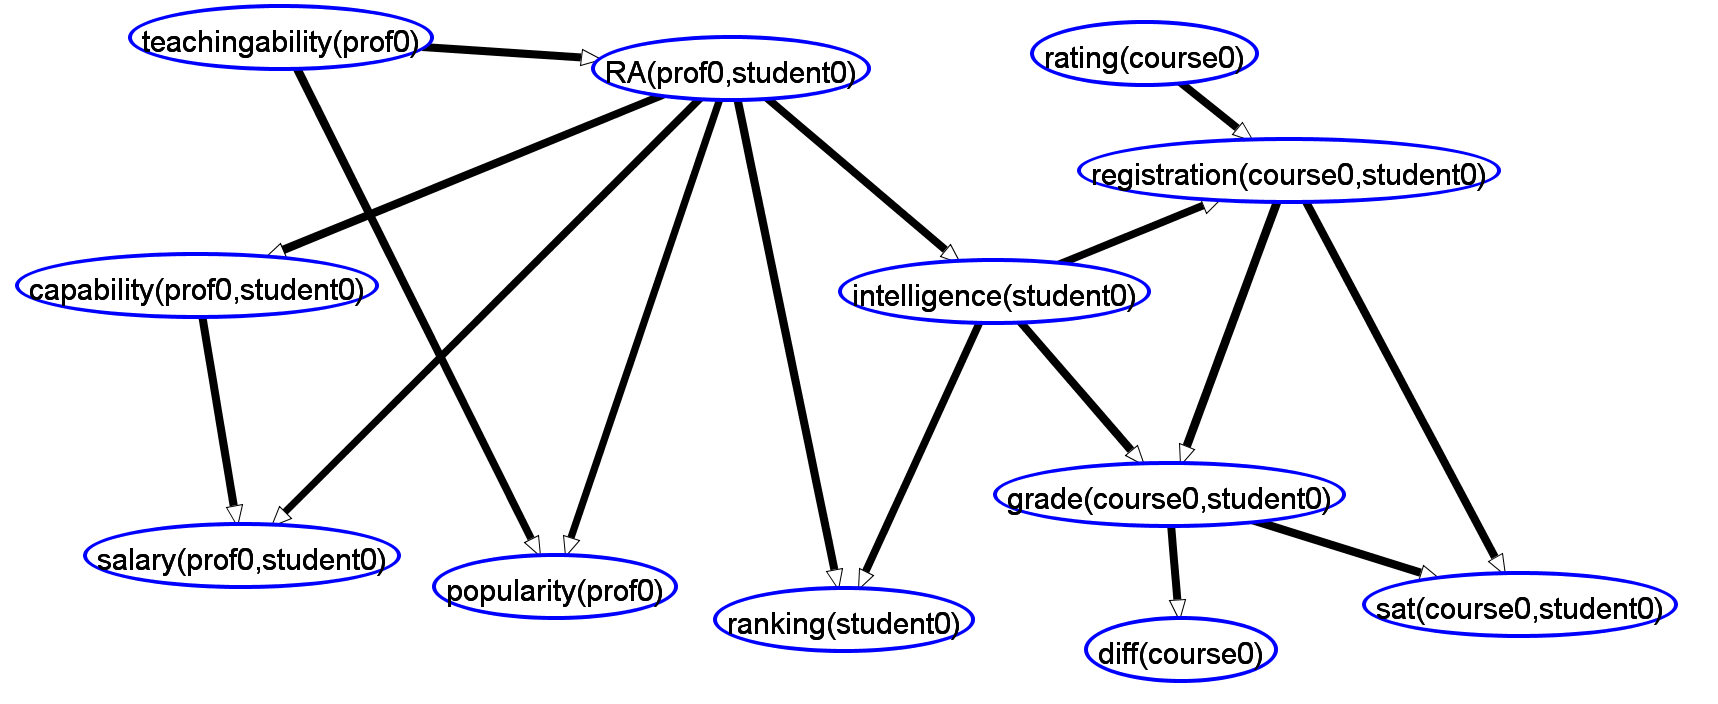
\includegraphics[width=7in,height=0.3\textheight]{unielwin.png}
%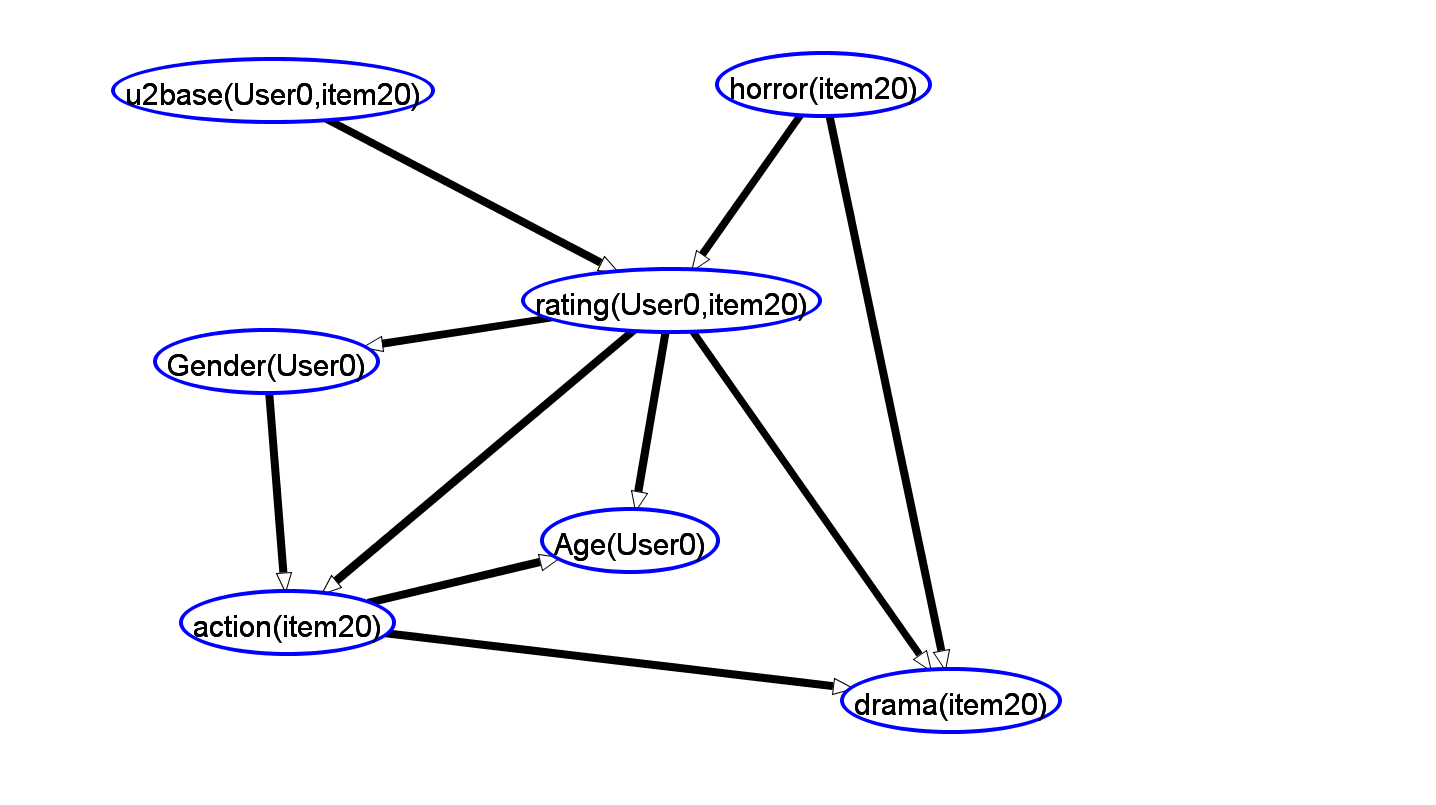
\includegraphics[width=7in,height=0.3\textheight]{movielens.png}
%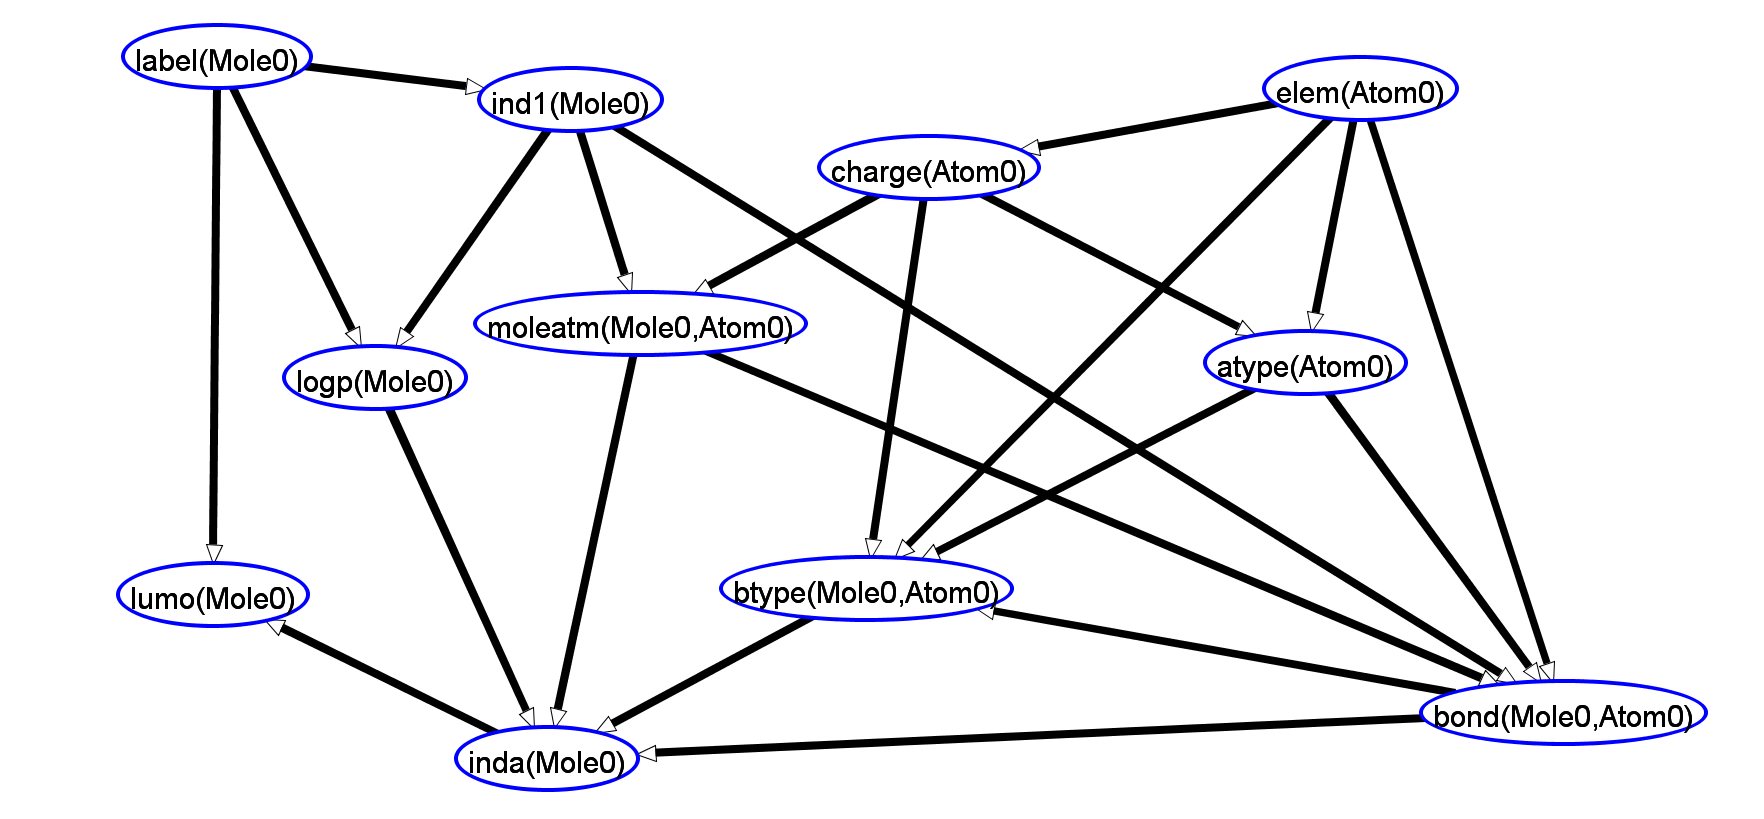
\includegraphics[width=7in,height=0.3\textheight]{muta.png}
%
%  \caption{Real Bayes Net Examples:.}
%   \label{fig:BN_Examplse}
%\end{figure*}


 



\section{Conclusion and Future Work} 

A key factor for scalable machine learning is fast access to sufficient statistics, which can be stored in contingency tables. We presented an algorithm for computing a joint contingency table for an entire relational database. The contingency table includes sufficient statistics for conjunctive queries that combine information from different database tables, and may contain any number of negative relationships. Sufficient statistics for negative relationships support learning correlations among relationships, that can be used for probabilistic reasoning about links in the relational structure. We present a dynamic program that extends a cache of sufficient statistics for positive relationships to a cache for negative relationships. The basis of the dynamic program is a subtraction method for obtaining query counts with $k+1$ negative relationships, from counts with only $k$ negative relationships. To derive the subtraction method, we introduced $\ct$-table algebra, an extension of relational algebra designed for computation with contingency tables. $\ct$-table algebra facilitates the efficient implementation of the dynamic program. 

The joint contingency table can be applied to learning a Bayes net structure that represents probabilistic dependencies across the entire database. The efficient computation of sufficient statistics allows the system to scale to large datasets (over 1M tuples) with fairly complex schemas. We find that a hierarchical lattice search strategy 
\cite{Schulte2012,Qian_LNAI_2014} performs better than simply using the joint contingency table, in terms of both learning time and model selection scores. 

In addition to computational efficiency, an attractive property of our system is that it applies to SQL-based databases in general, and requires almost no configuration input from the  user to prepare a target database for analysis. We achieve this generality by extracting from the system metadata information about the random variables that are the target of statististical analysis.  


\emph{Future Work.} Our dynamic program scales well with the number of rows, but not with the number of columns and relationships in the data tables. This is because the size of the joint contingency table grows exponentially with the number of random variables in the table. One approach would be to apply the dynamic programming algorithm only  up to a relatively small relationship chain length. A sufficient chain length could be specified by the user or determined by a learning algorithm. Another approach is to use the virtual join algorithm with postcounting: Rather than precompute large contingency tables for a large set of random variables prior to learning, compute many small contingency tables for  small subsets of variables. In a postcounting approach, generating a contingency table for a target set of variables is a service that can be called dynamically in the executation of a learning program  [chinese paper, also Friedman ``massive datasets'']. 

A cache of sufficient statistics can be applied to many learning problems, in addition to learning Bayes net structure. Examples include relational classification and link prediction methods. Another potential application is in probabilistic first-order inference. Such inferences often require sufficient statistics (parfactors) defined with respect to one or more specified individuals (e.g., the number of user $u$'s male friends). It is easy to extend our virtual join algorithm to compute sufficient statistics for specified individuals. 

In sum, our virtual join algorithm efficiently computes query counts for negative relationships. These sufficient statistics supports a scalable statistical analysis of  dependencies among both relationships and attributes in a relational database.



%ACKNOWLEDGMENTS are optional
\section{Acknowledgments}

This research was supported by a Discovery grant to Oliver Schulte by the Natural Sciences and Engineering Research Council of Canada. 
Zhensong Qian was supported by a grant from the China Scholarship Council.
%[preliminary results about We thank the organizers for providing a discussion venue, and the anonymous reviewers for constructive criticism.


% The following two commands are all you need in the
% initial runs of your .tex file to
% produce the bibliography for the citations in your paper.
\bibliographystyle{abbrv}
\bibliography{master} 

 % vldb_sample.bib is the name of the Bibliography in this case
% You must have a proper ".bib" file
%  and remember to run:
% latex bibtex latex latex
% to resolve all references

%\subsection{References}

%APPENDIX is optional.
% ****************** APPENDIX **************************************
% Example of an appendix; typically would start on a new page
%pagebreak

%\begin{appendix}
%You can use an appendix for optional proofs or details of your evaluation which are not absolutely necessary to the core understanding of your paper. 
%
%\section{Final Thoughts on Good Layout}
%Please use readable font sizes in the figures and graphs. Avoid tempering with the correct border values, and the spacing (and format) of both text and captions of the PVLDB format (e.g. captions are bold).
%
%At the end, please check for an overall pleasant layout, e.g. by ensuring a readable and logical positioning of any floating figures and tables. Please also check for any line overflows, which are only allowed in extraordinary circumstances (such as wide formulas or URLs where a line wrap would be counterintuitive).
%
%Use the \texttt{balance} package together with a \texttt{\char'134 balance} command at the end of your document to ensure that the last page has balanced (i.e. same length) columns.
%
%\end{appendix}



\end{document}
